%**************************************%
%*    Generated from PreTeXt source   *%
%*    on 2018-08-30T11:03:17-05:00    *%
%*                                    *%
%*   http://mathbook.pugetsound.edu   *%
%*                                    *%
%**************************************%
\documentclass[10pt,]{article}
%% Custom Preamble Entries, early (use latex.preamble.early)
%% Default LaTeX packages
%%   1.  always employed (or nearly so) for some purpose, or
%%   2.  a stylewriter may assume their presence
\usepackage{geometry}
%% Some aspects of the preamble are conditional,
%% the LaTeX engine is one such determinant
\usepackage{ifthen}
%% etoolbox has a variety of modern conveniences
\usepackage{etoolbox}
\usepackage{ifxetex,ifluatex}
%% Raster graphics inclusion
\usepackage{graphicx}
%% Color support, xcolor package
%% Always loaded, for: add/delete text, author tools
%% Here, since tcolorbox loads tikz, and tikz loads xcolor
\PassOptionsToPackage{usenames,dvipsnames,svgnames,table}{xcolor}
\usepackage{xcolor}
%% Colored boxes, and much more, though mostly styling
%% skins library provides "enhanced" skin, employing tikzpicture
%% vignette library provides fancy shaded frames
%% boxes may be configured as "breakable" or "unbreakable"
%% "raster" controls grids of boxes, aka side-by-side
\usepackage{tcolorbox}
\tcbuselibrary{skins}
\tcbuselibrary{vignette}
\tcbuselibrary{breakable}
\tcbuselibrary{raster}
%% xparse allows the construction of more robust commands,
%% this is a necessity for isolating styling and behavior
%% The tcolorbox library of the same name loads the base library
\tcbuselibrary{xparse}
%% Hyperref should be here, but likes to be loaded late
%%
%% Inline math delimiters, \(, \), need to be robust
%% 2016-01-31:  latexrelease.sty  supersedes  fixltx2e.sty
%% If  latexrelease.sty  exists, bugfix is in kernel
%% If not, bugfix is in  fixltx2e.sty
%% See:  https://tug.org/TUGboat/tb36-3/tb114ltnews22.pdf
%% and read "Fewer fragile commands" in distribution's  latexchanges.pdf
\IfFileExists{latexrelease.sty}{}{\usepackage{fixltx2e}}
%% Text height identically 9 inches, text width varies on point size
%% See Bringhurst 2.1.1 on measure for recommendations
%% 75 characters per line (count spaces, punctuation) is target
%% which is the upper limit of Bringhurst's recommendations
\geometry{letterpaper,total={340pt,9.0in}}
%% Custom Page Layout Adjustments (use latex.geometry)
%% This LaTeX file may be compiled with pdflatex, xelatex, or lualatex
%% The following provides engine-specific capabilities
%% Generally, xelatex and lualatex will do better languages other than US English
%% You can pick from the conditional if you will only ever use one engine
\ifthenelse{\boolean{xetex} \or \boolean{luatex}}{%
%% begin: xelatex and lualatex-specific configuration
%% fontspec package will make Latin Modern (lmodern) the default font
\ifxetex\usepackage{xltxtra}\fi
\usepackage{fontspec}
%% realscripts is the only part of xltxtra relevant to lualatex 
\ifluatex\usepackage{realscripts}\fi
%% 
%% Extensive support for other languages
\usepackage{polyglossia}
%% Main document language is US English
\setdefaultlanguage{english}
%% Spanish
\setotherlanguage{spanish}
%% Vietnamese
\setotherlanguage{vietnamese}
%% end: xelatex and lualatex-specific configuration
}{%
%% begin: pdflatex-specific configuration
%% translate common Unicode to their LaTeX equivalents
%% Also, fontenc with T1 makes CM-Super the default font
%% (\input{ix-utf8enc.dfu} from the "inputenx" package is possible addition (broken?)
\usepackage[T1]{fontenc}
\usepackage[utf8]{inputenc}
%% end: pdflatex-specific configuration
}
%% Symbols, align environment, bracket-matrix
\usepackage{amsmath}
\usepackage{amssymb}
%% allow page breaks within display mathematics anywhere
%% level 4 is maximally permissive
%% this is exactly the opposite of AMSmath package philosophy
%% there are per-display, and per-equation options to control this
%% split, aligned, gathered, and alignedat are not affected
\allowdisplaybreaks[4]
%% allow more columns to a matrix
%% can make this even bigger by overriding with  latex.preamble.late  processing option
\setcounter{MaxMatrixCols}{30}
%%
%% Semantic Macros
%% To preserve meaning in a LaTeX file
%% Only defined here if required in this document
%% Used for inline definitions of terms
\newcommand{\terminology}[1]{\textbf{#1}}
%% Subdivision Numbering, Chapters, Sections, Subsections, etc
%% Subdivision numbers may be turned off at some level ("depth")
%% A section *always* has depth 1, contrary to us counting from the document root
%% The latex default is 3.  If a larger number is present here, then
%% removing this command may make some cross-references ambiguous
%% The precursor variable $numbering-maxlevel is checked for consistency in the common XSL file
\setcounter{secnumdepth}{3}
%% begin: General AMS environment setup
%% Environments built with amsthm package
\usepackage{amsthm}
%% Numbering for Theorems, Conjectures, Examples, Figures, etc
%% Controlled by  numbering.theorems.level  processing parameter
%% Numbering: all theorem-like numbered consecutively
%% i.e. Corollary 4.3 follows Theorem 4.2
%% Always need some theorem environment to set base numbering scheme
%% even if document has no theorems (but has other environments)
%% Create a never-used style first, always
%% simply to provide a global counter to use, namely "cthm"
\newtheorem{cthm}{BadTheoremStringName}[section]
%% end: General AMS environment setup
%%
%% tcolorbox, with styles, for THEOREM-LIKE
%%
%% theorem: fairly simple numbered block/structure
\tcbset{ theoremstyle/.style={size=minimal, boxrule=-0.3pt, frame empty, colback=white, colbacktitle=white, coltitle=black, fonttitle=\normalfont\bfseries, attach title to upper, after title={\space}, } }
\newtcolorbox[use counter=cthm, number within=section]{theorem}[3]{title={{Theorem~\thetcbcounter\notblank{#1#2}{\space}{}\notblank{#1}{\space#1}{}\notblank{#2}{\space(#2)}{}}}, label=#3, breakable, fontupper=\itshape, theoremstyle, }
%% proposition: fairly simple numbered block/structure
\tcbset{ propositionstyle/.style={size=minimal, boxrule=-0.3pt, frame empty, colback=white, colbacktitle=white, coltitle=black, fonttitle=\normalfont\bfseries, attach title to upper, after title={\space}, } }
\newtcolorbox[use counter=cthm, number within=section]{proposition}[3]{title={{Proposition~\thetcbcounter\notblank{#1#2}{\space}{}\notblank{#1}{\space#1}{}\notblank{#2}{\space(#2)}{}}}, label=#3, breakable, fontupper=\itshape, propositionstyle, }
%%
%% tcolorbox, with styles, for DEFINITION-LIKE
%%
%% definition: fairly simple numbered block/structure
\tcbset{ definitionstyle/.style={size=minimal, boxrule=-0.3pt, frame empty, colback=white, colbacktitle=white, coltitle=black, fonttitle=\normalfont\bfseries, attach title to upper, after title={\space}, after upper={\hfill{}\(\lozenge\)}, } }
\newtcolorbox[use counter=cthm, number within=section]{definition}[2]{title={{Definition~\thetcbcounter\notblank{#1}{\space\space#1}{}}}, label=#2, breakable, definitionstyle, }
%%
%% tcolorbox, with styles, for EXAMPLE-LIKE
%%
%% example: fairly simple numbered block/structure
\tcbset{ examplestyle/.style={size=minimal, boxrule=-0.3pt, frame empty, colback=white, colbacktitle=white, coltitle=black, fonttitle=\normalfont\bfseries, attach title to upper, after title={\space}, after upper={\hfill{}\(\square\)}, } }
\newtcolorbox[use counter=cthm, number within=section]{example}[2]{title={{Example~\thetcbcounter\notblank{#1}{\space\space#1}{}}}, label=#2, breakable, examplestyle, }
%% Localize LaTeX supplied names (possibly none)
\renewcommand*{\appendixname}{Appendix}
\renewcommand*{\abstractname}{Abstract}
%% Figures, Tables, Listings, Named Lists, Floats
%% The [H]ere option of the float package fixes floats in-place,
%% in deference to web usage, where floats are totally irrelevant
%% You can remove some of this setup, to restore standard LaTeX behavior
%% HOWEVER, numbering of figures/tables AND theorems/examples/remarks, etc
%% may de-synchronize with the numbering in the HTML version
%% You can remove the "placement={H}" option to allow flotation and
%% preserve numbering, BUT the numbering may then appear "out-of-order"
%% Floating environments: http://tex.stackexchange.com/questions/95631/
\usepackage{float}
\usepackage{newfloat}
\usepackage{caption}%% Adjust stock figure environment so that it no longer floats
\SetupFloatingEnvironment{figure}{fileext=lof,placement={H},within=section,name=Figure}
\captionsetup[figure]{labelfont=bf}
%% http://tex.stackexchange.com/questions/16195
\makeatletter
\let\c@figure\c@cthm
\makeatother
%% Footnote Numbering
%% We reset the footnote counter, as given by numbering.footnotes.level
\makeatletter\@addtoreset{footnote}{section}\makeatother
%% More flexible list management, esp. for references
%% But also for specifying labels (i.e. custom order) on nested lists
\usepackage{enumitem}
%% hyperref driver does not need to be specified, it will be detected
\usepackage{hyperref}
%% configure hyperref's  \url  to match listings' inline verbatim
\renewcommand\UrlFont{\small\ttfamily}
%% Hyperlinking active in PDFs, all links solid and blue
\hypersetup{colorlinks=true,linkcolor=blue,citecolor=blue,filecolor=blue,urlcolor=blue}
\hypersetup{pdftitle={Intro to Topology}}
%% If you manually remove hyperref, leave in this next command
\providecommand\phantomsection{}
%% If tikz has been loaded, replace ampersand with \amp macro
%% extpfeil package for certain extensible arrows,
%% as also provided by MathJax extension of the same name
%% NB: this package loads mtools, which loads calc, which redefines
%%     \setlength, so it can be removed if it seems to be in the 
%%     way and your math does not use:
%%     
%%     \xtwoheadrightarrow, \xtwoheadleftarrow, \xmapsto, \xlongequal, \xtofrom
%%     
%%     we have had to be extra careful with variable thickness
%%     lines in tables, and so also load this package late
\usepackage{extpfeil}
%% Custom Preamble Entries, late (use latex.preamble.late)
%% Begin: Author-provided packages
%% (From  docinfo/latex-preamble/package  elements)
%% End: Author-provided packages
%% Begin: Author-provided macros
%% (From  docinfo/macros  element)
%% Plus three from MBX for XML characters
\newcommand{\tuple}[1]{\langle #1 \rangle}
\newcommand{\mb}{\mathbb}
\newcommand{\mc}{\mathcal}
\newcommand{\cl}{\operatorname{cl}}
\newcommand{\int}{\operatorname{int}}
\newcommand{\ext}{\operatorname{ext}}
\newcommand{\bd}{\operatorname{bd}}
\newcommand{\setBuilder}[2]{\left\{#1:#2\right\}}
\newcommand{\setList}[1]{\left\{#1\right\}}
\newcommand{\lt}{<}
\newcommand{\gt}{>}
\newcommand{\amp}{&}
%% End: Author-provided macros
%% Title page information for article
\title{Intro to Topology}
\author{Steven Clontz\\
University of South Alabama
}
\date{August 30, 2018}
\begin{document}
%% Target for xref to top-level element is document start
\hypertarget{index}{}
\maketitle
\thispagestyle{empty}
\begin{abstract}
\hypertarget{p-1}{}%
These are course notes for an introductory course for general topology, to be used in an inquiry-based learning classroom.%
\par
\hypertarget{p-2}{}%
Some of this content has been adapted from Michel Smith's undergraduate topology notes, used with permission.%
\par
\hypertarget{p-3}{}%
Dr. Clontz's website for students is \url{https://prof.clontz.org}. His personal website is \url{https://clontz.org}.%
\end{abstract}
\hypertarget{p-4}{}%
These are course notes for an introductory course for general topology, to be used in an inquiry-based learning classroom.%
%
%
\typeout{************************************************}
\typeout{Section 1 Curves and Surfaces}
\typeout{************************************************}
%
\section[{Curves and Surfaces}]{Curves and Surfaces}\label{section-surfaces}
\hypertarget{p-5}{}%
In this section, we will develop an intuition for a topological space and the purpose of topology by investigating two natural examples of topological spaces: curves and surfaces.%
\par
\hypertarget{p-6}{}%
Unlike the rest of these notes, this section is not meant to be studied rigorously. (For example, what do I mean by ``locally looks like'' in \hyperref[curve-defn]{Definition~\ref{curve-defn}}?)  However, many of these ideas will return later in the course and be handled more carefully.%
\begin{definition}{}{curve-defn}%
\hypertarget{p-7}{}%
A \terminology{curve} is a set of points such that for every point in the set, the set locally looks like a (possibly bent or curved) copy of the real line \(\mathbb R\) or the half line \(\mathbb R^*=\{x\in\mathbb R:x\geq 0\}\).%
\end{definition}
\hypertarget{p-8}{}%
For example, \hyperref[circle-fig]{Figure~\ref{circle-fig}}, \hyperref[figure-parabola]{Figure~\ref{figure-parabola}}, and \hyperref[figure-helix]{Figure~\ref{figure-helix}} are all examples of curves in two or three-dimensional Euclidean space.%
\begin{figure}
\centering
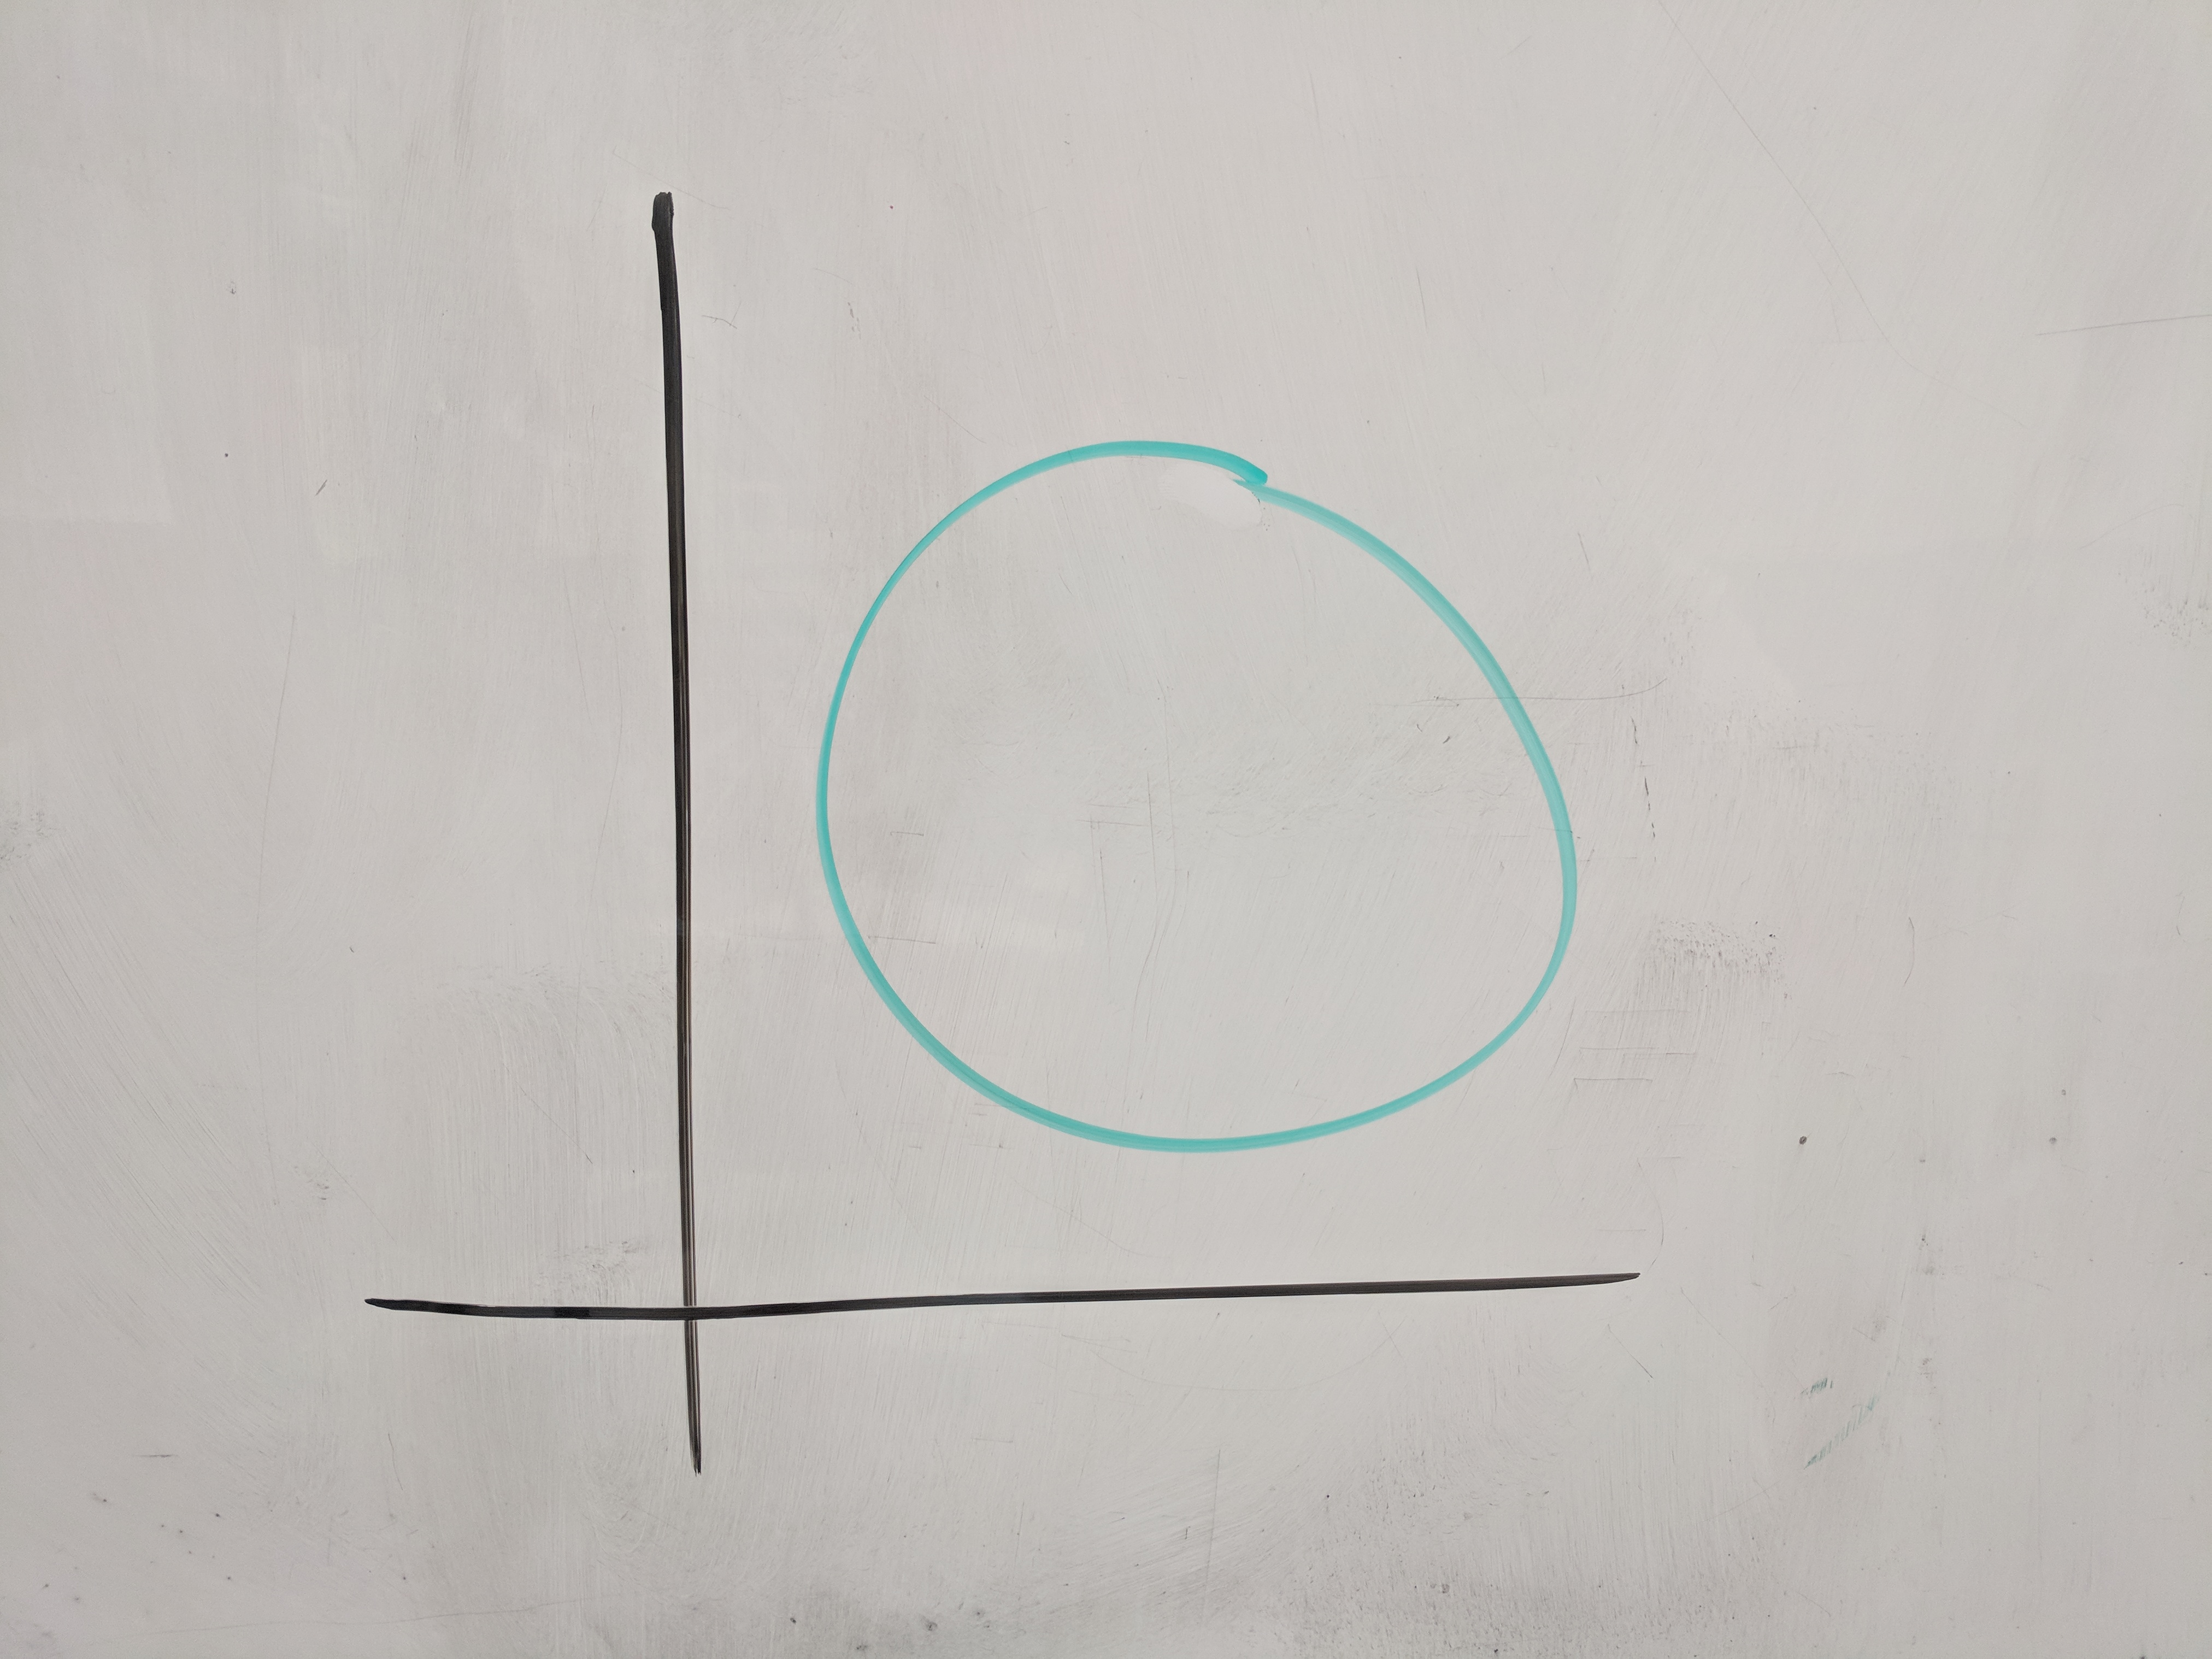
\includegraphics[width=1\linewidth]{images/circle.jpg}
\caption{A circle\label{circle-fig}}
\end{figure}
\begin{figure}
\centering
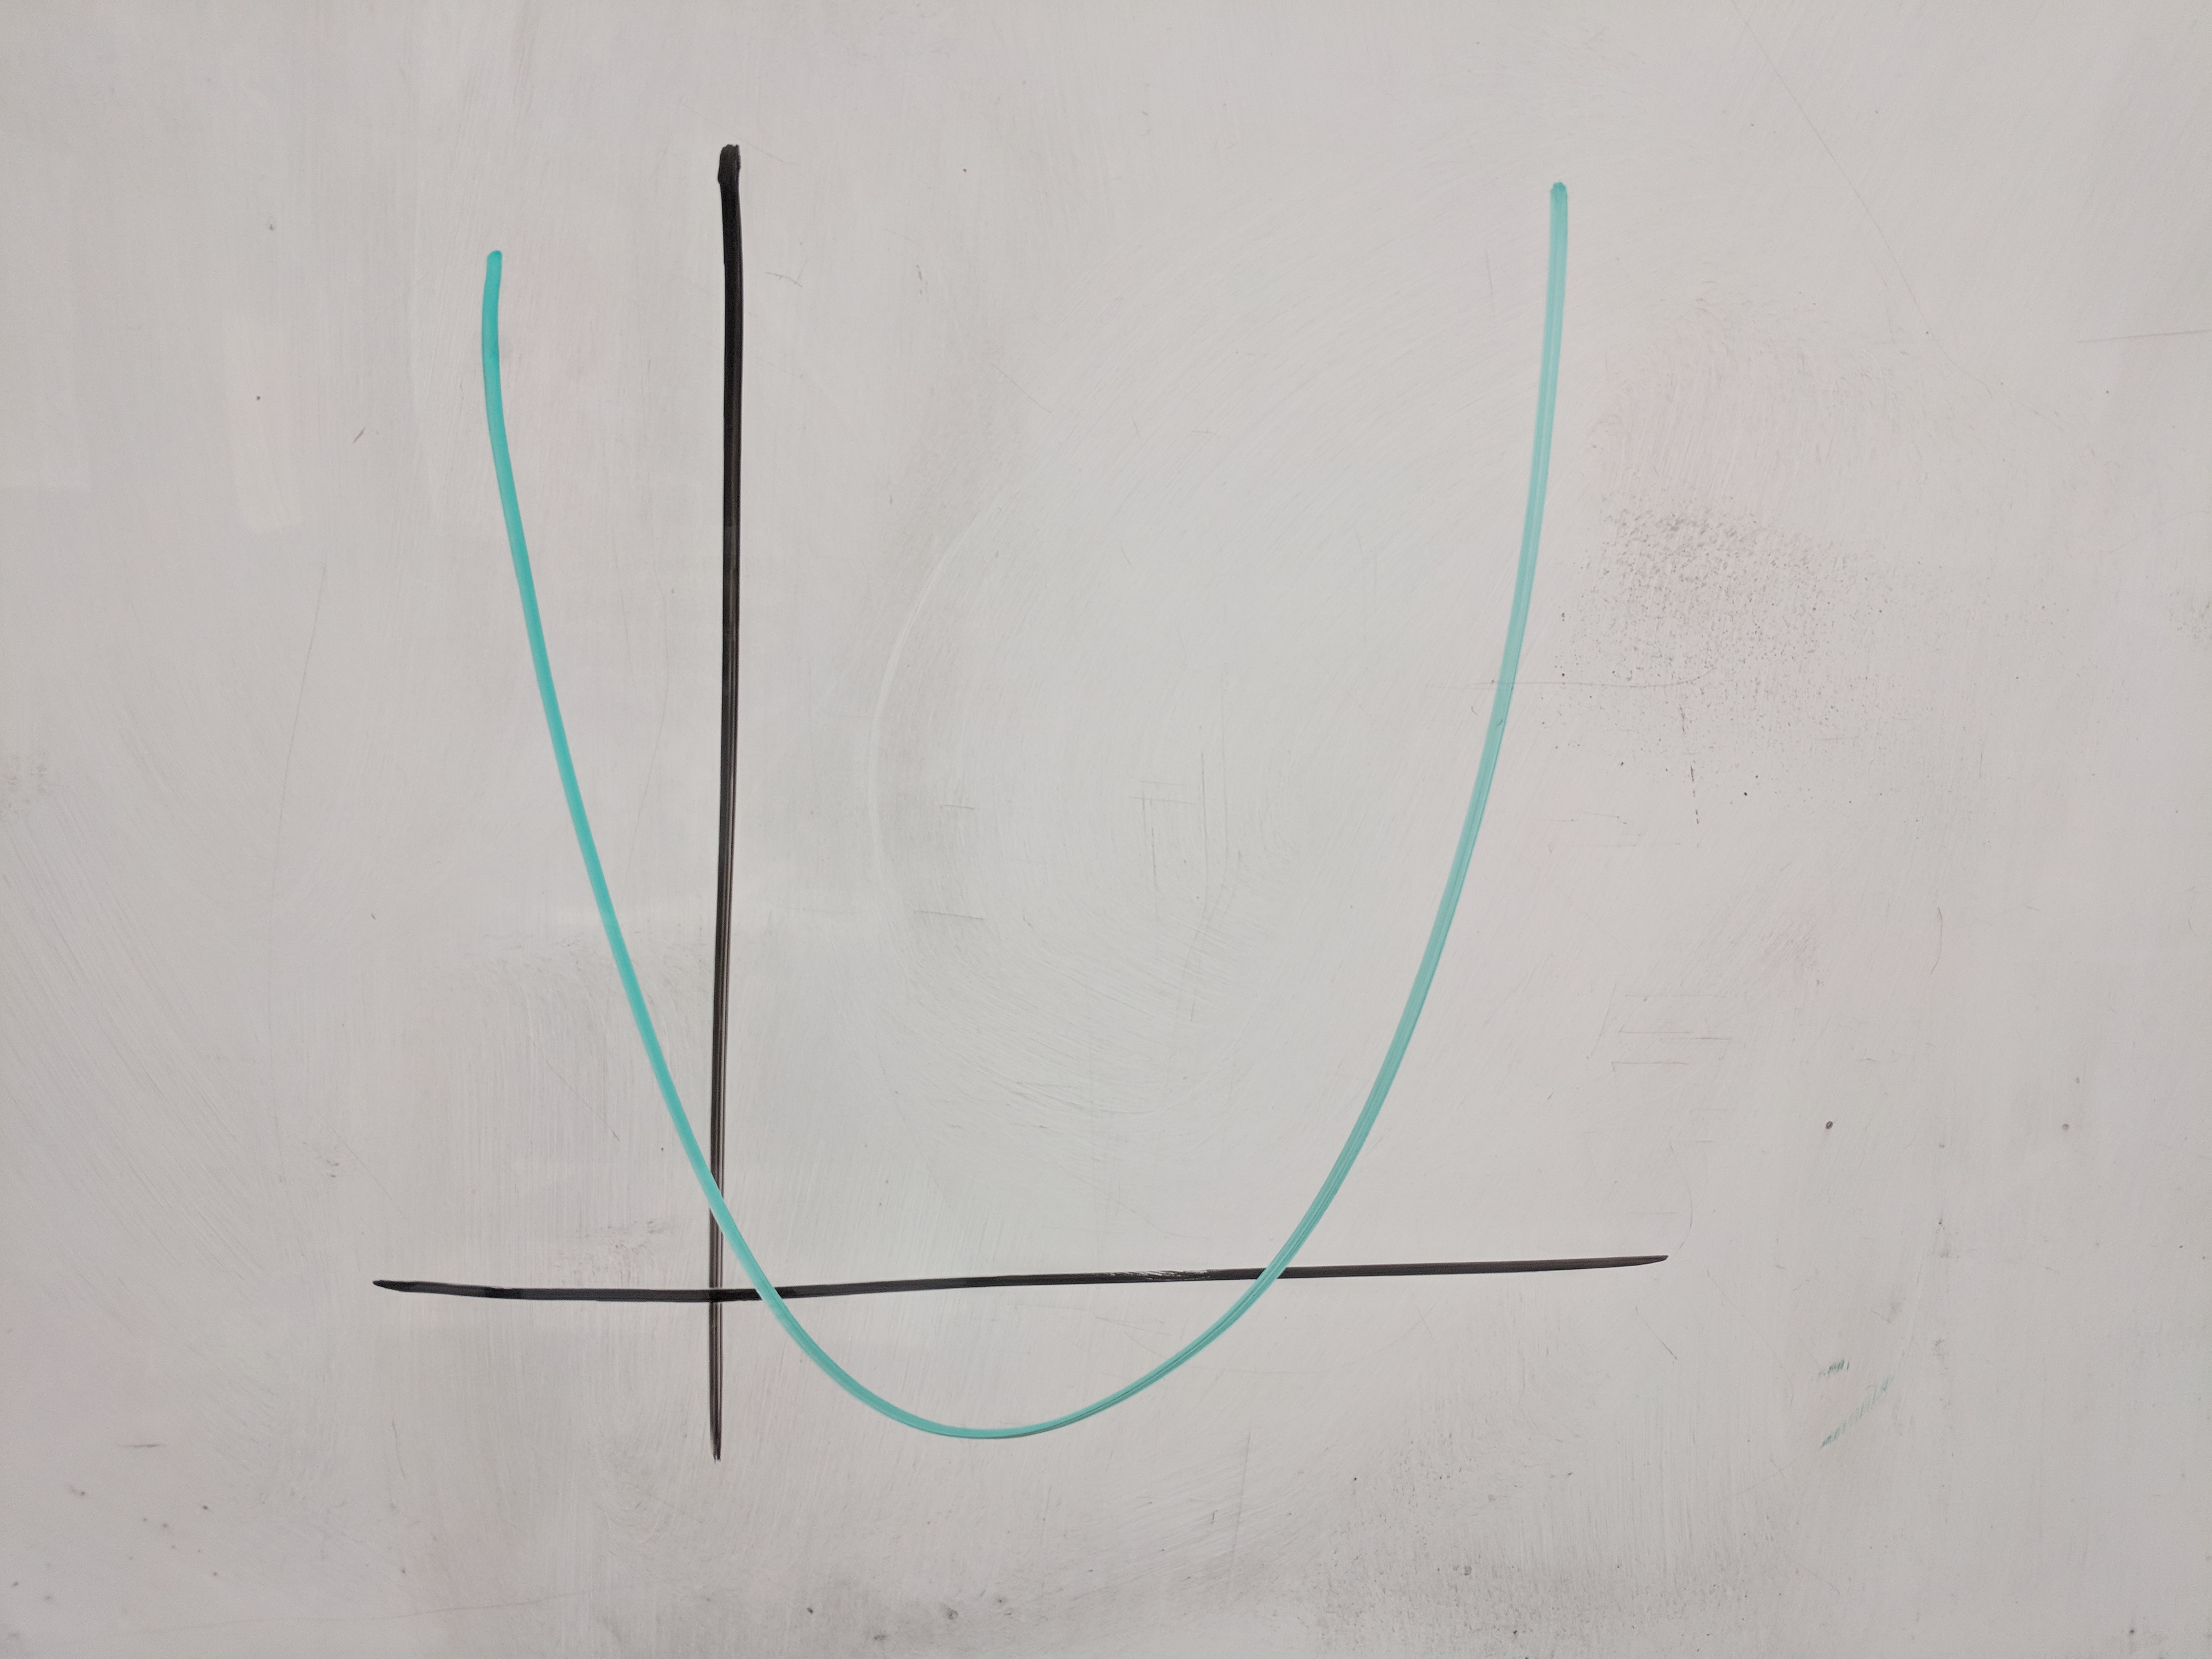
\includegraphics[width=1\linewidth]{images/parabola.jpg}
\caption{A parabola\label{figure-parabola}}
\end{figure}
\begin{figure}
\centering
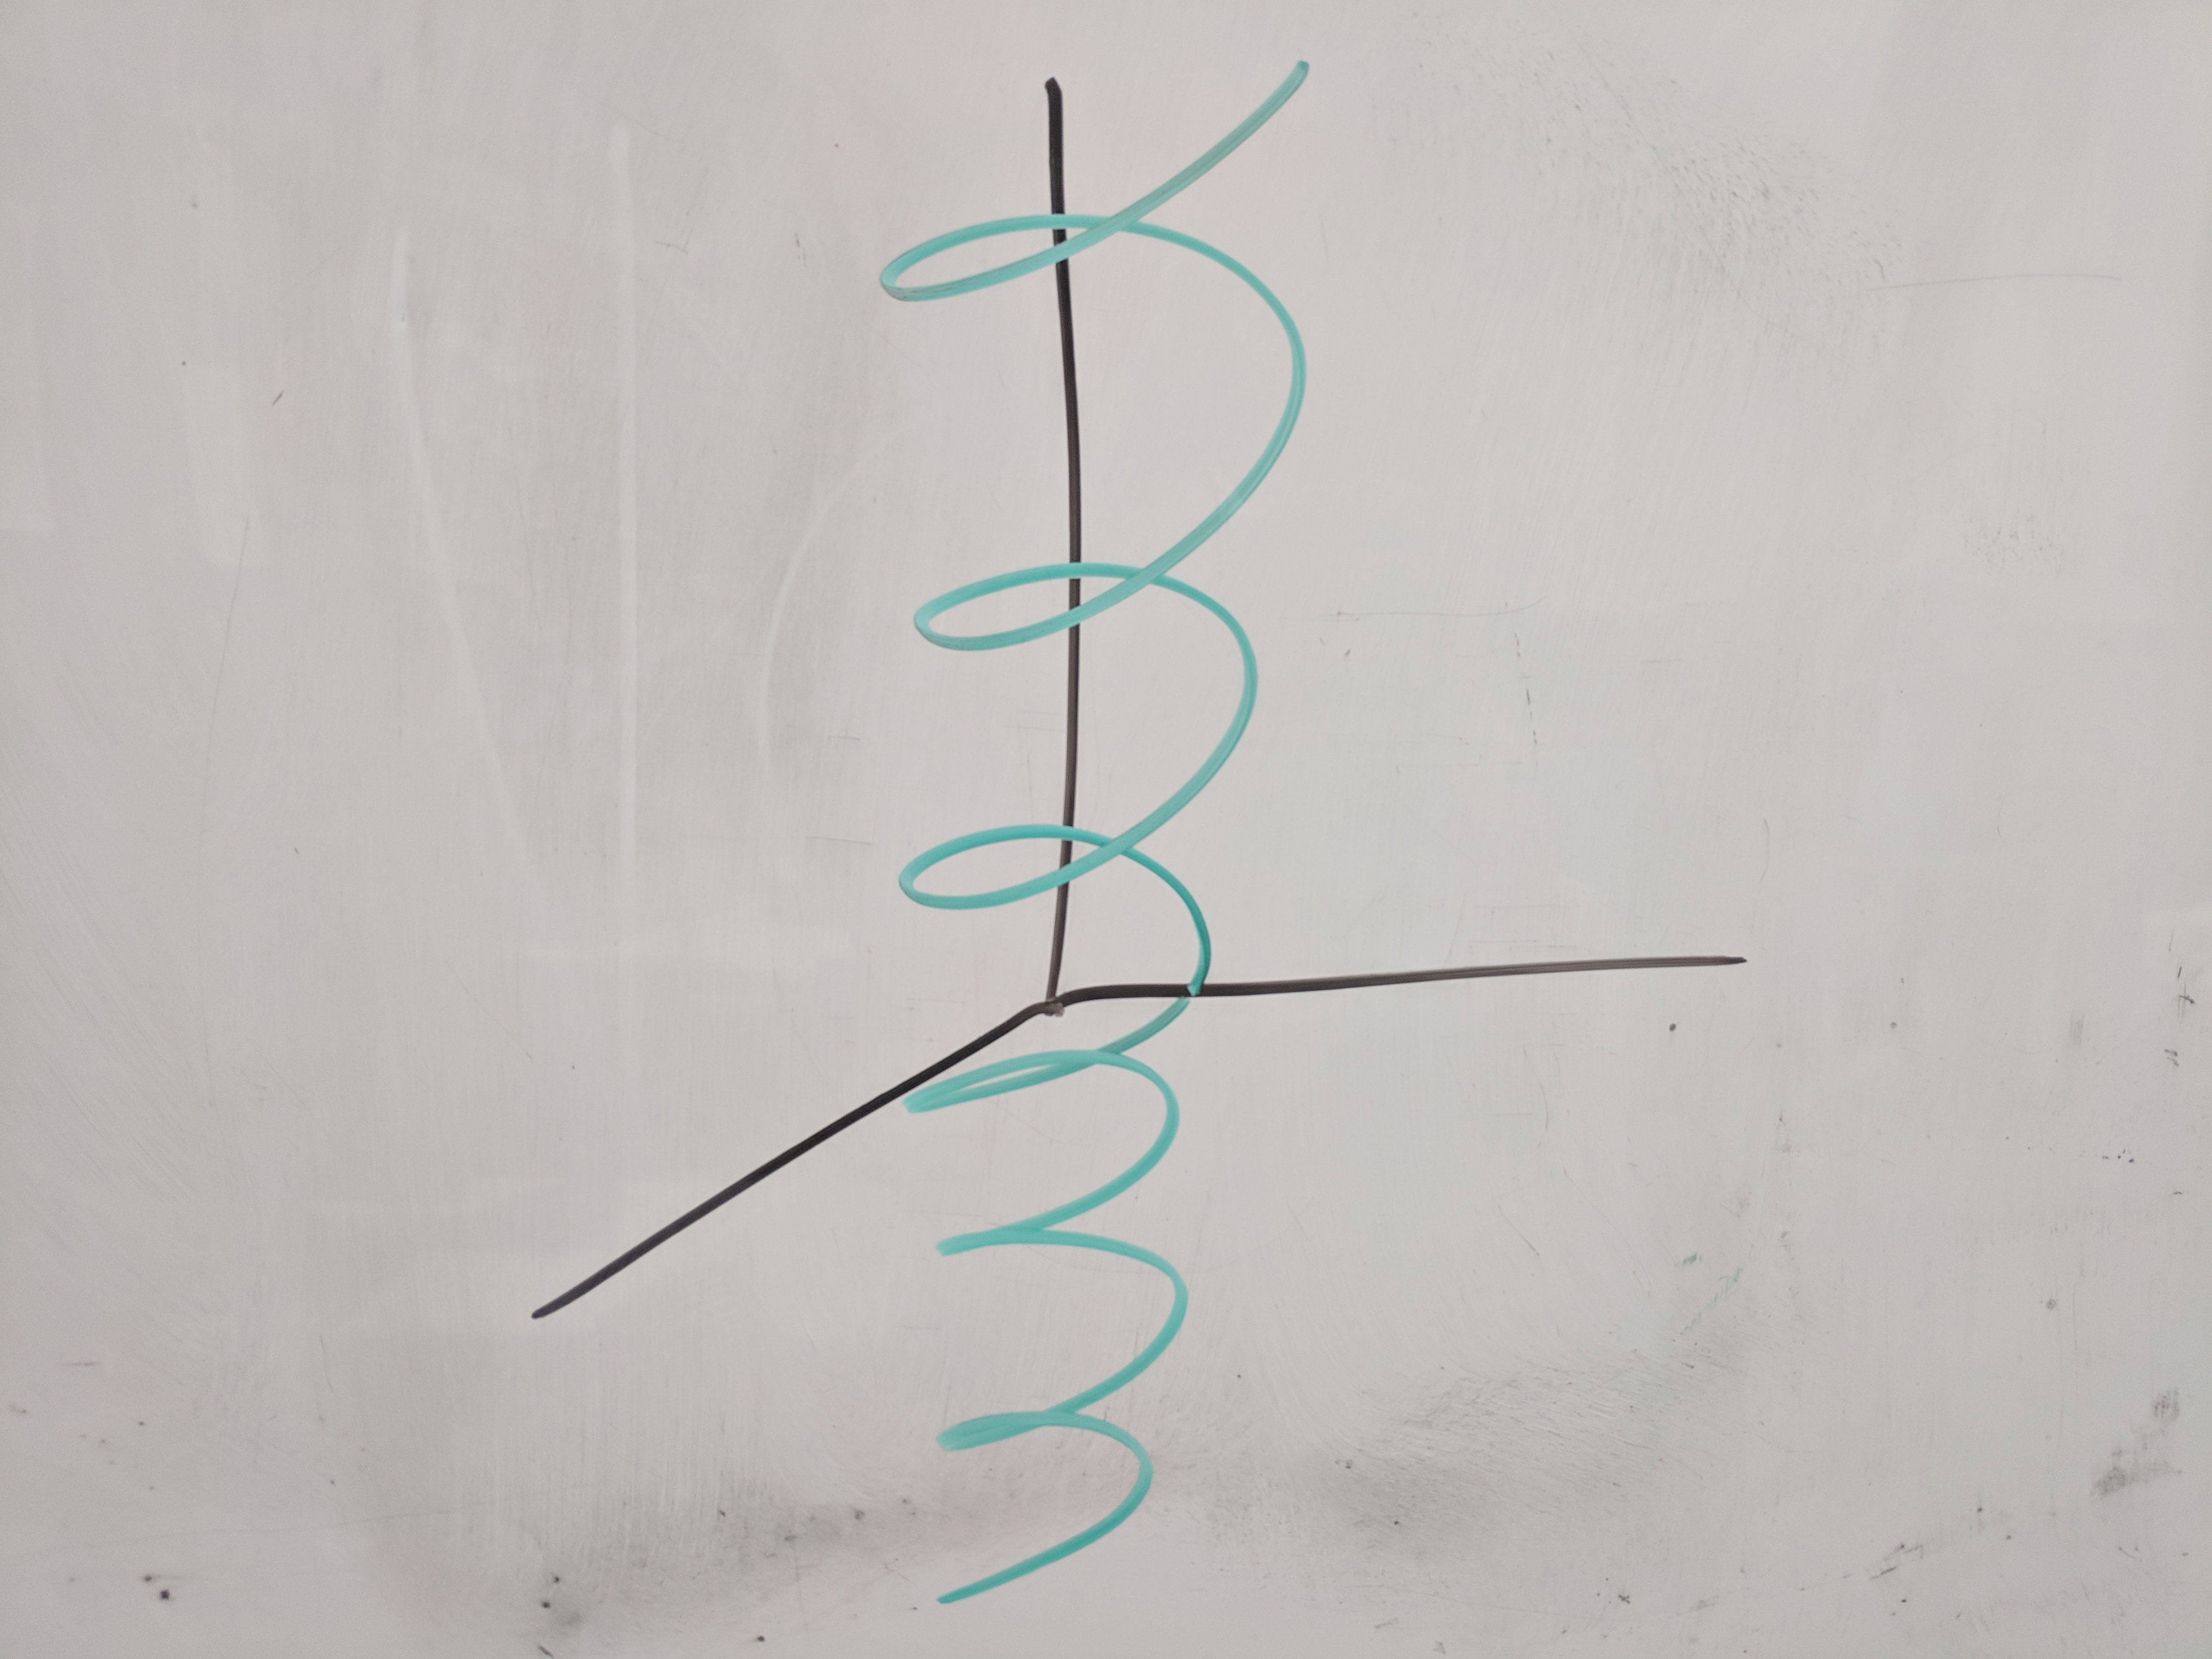
\includegraphics[width=1\linewidth]{images/helix.jpg}
\caption{A helix\label{figure-helix}}
\end{figure}
\hypertarget{p-9}{}%
Note the following differences between \hyperref[circle-fig]{Figure~\ref{circle-fig}} and \hyperref[figure-parabola]{Figure~\ref{figure-parabola}}:%
\leavevmode%
\begin{itemize}[label=\textbullet]
\item{}Removing a point from \hyperref[figure-parabola]{Figure~\ref{figure-parabola}} would split it into two disconnected parts, but \hyperref[circle-fig]{Figure~\ref{circle-fig}} would remain connected after a point is removed.%
\item{}\hyperref[circle-fig]{Figure~\ref{circle-fig}} is bounded while \hyperref[figure-parabola]{Figure~\ref{figure-parabola}} extends unboundedly. \footnote{This topological distinction makes sense as both are closed subsets of \(\mathbb R^2\); see \hyperref[section-compactness]{Section~\ref{section-compactness}} for more info.\label{fn-1}}%
\end{itemize}
\hypertarget{p-10}{}%
These differences would remain no matter how the curves were stretched or bent. However, while there are certainly geometrical differences beteween \hyperref[figure-parabola]{Figure~\ref{figure-parabola}} and \hyperref[figure-helix]{Figure~\ref{figure-helix}}, they are in a certain sense the same object that has been bent or stretched into a different shape.%
\begin{definition}{}{definition-2}%
\hypertarget{p-11}{}%
Two objects are said to be \terminology{topologically equivalent} or \terminology{homeomorphic} if one may be bent or stretched into the shape of the other.%
\end{definition}
\hypertarget{p-12}{}%
So this means that all geometrically similar shapes are homeomorphic (as in \hyperref[figure-similar-triangles]{Figure~\ref{figure-similar-triangles}}), but we also use the idea of homeomorphism to compare other objects in our daily lives.%
\par
\hypertarget{p-13}{}%
For example, while many of them are not curves by our definition, the letters of the alphabet may be considered as topological objects. \hyperref[figure-letter-a]{Figure~\ref{figure-letter-a}} illustrates several homeomorphic expressions of the letter ``A''.%
\begin{figure}
\centering
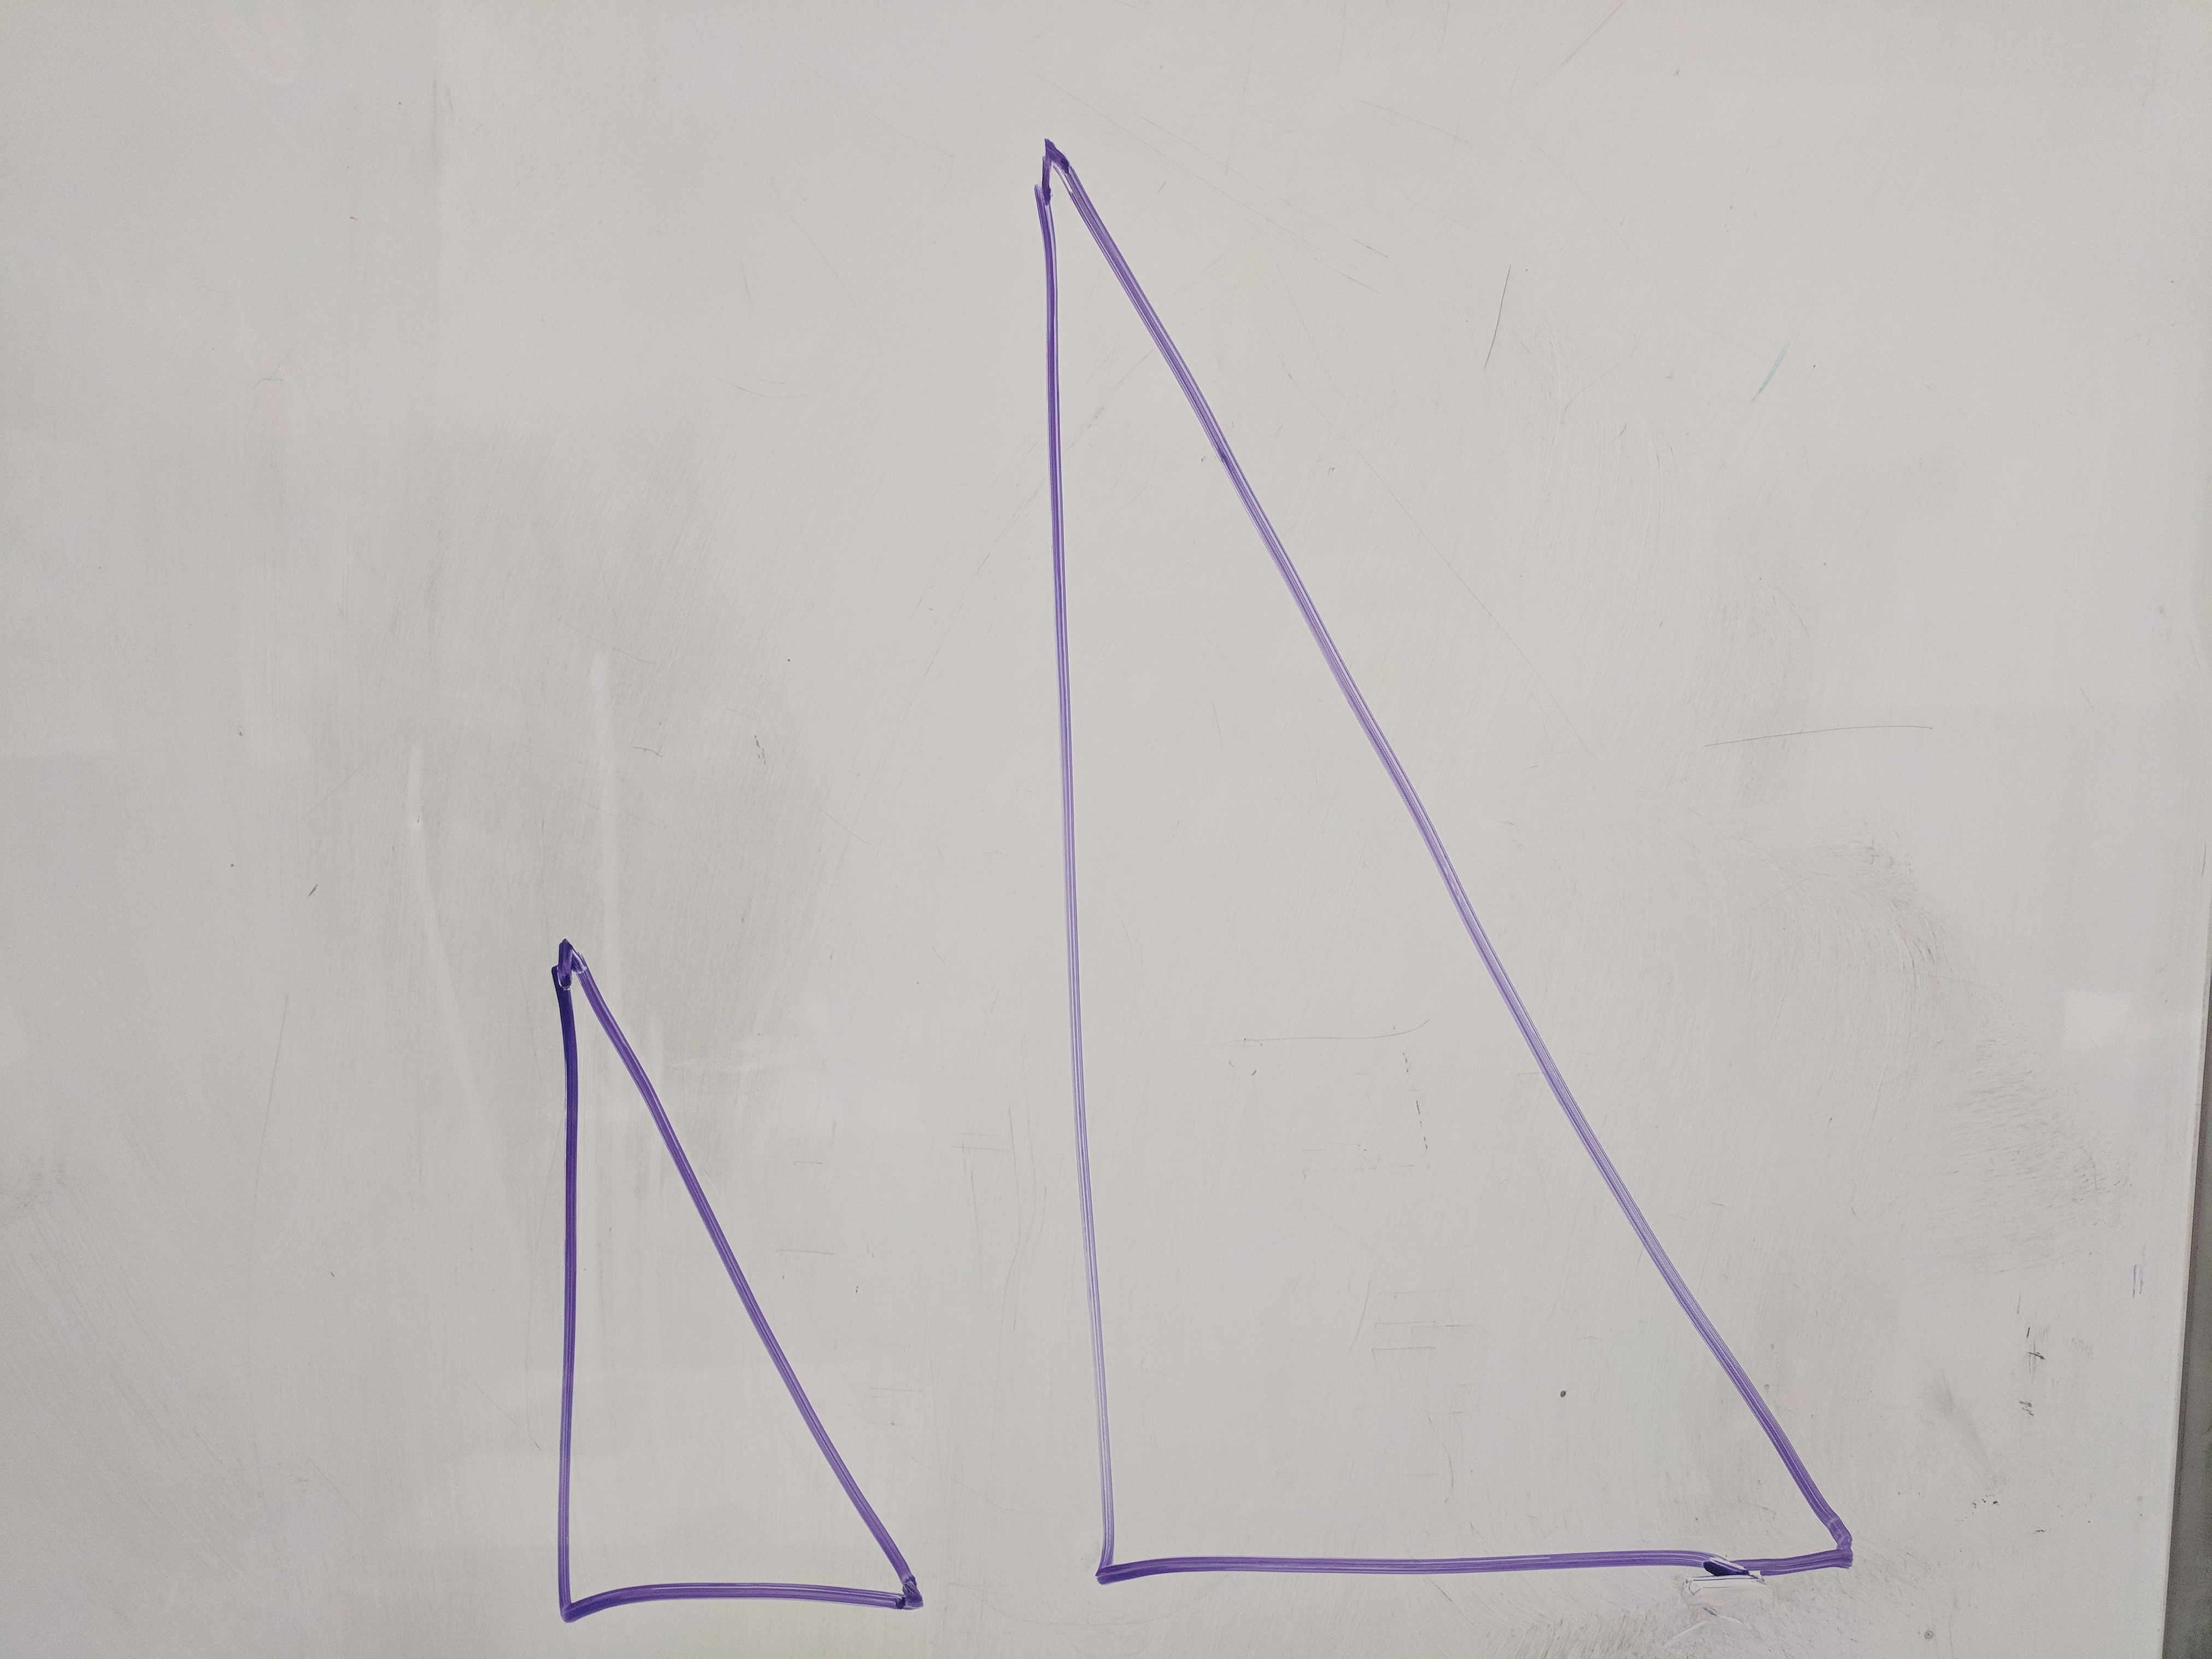
\includegraphics[width=1\linewidth]{images/similar-triangles.jpg}
\caption{Two similar triangles\label{figure-similar-triangles}}
\end{figure}
\begin{figure}
\centering
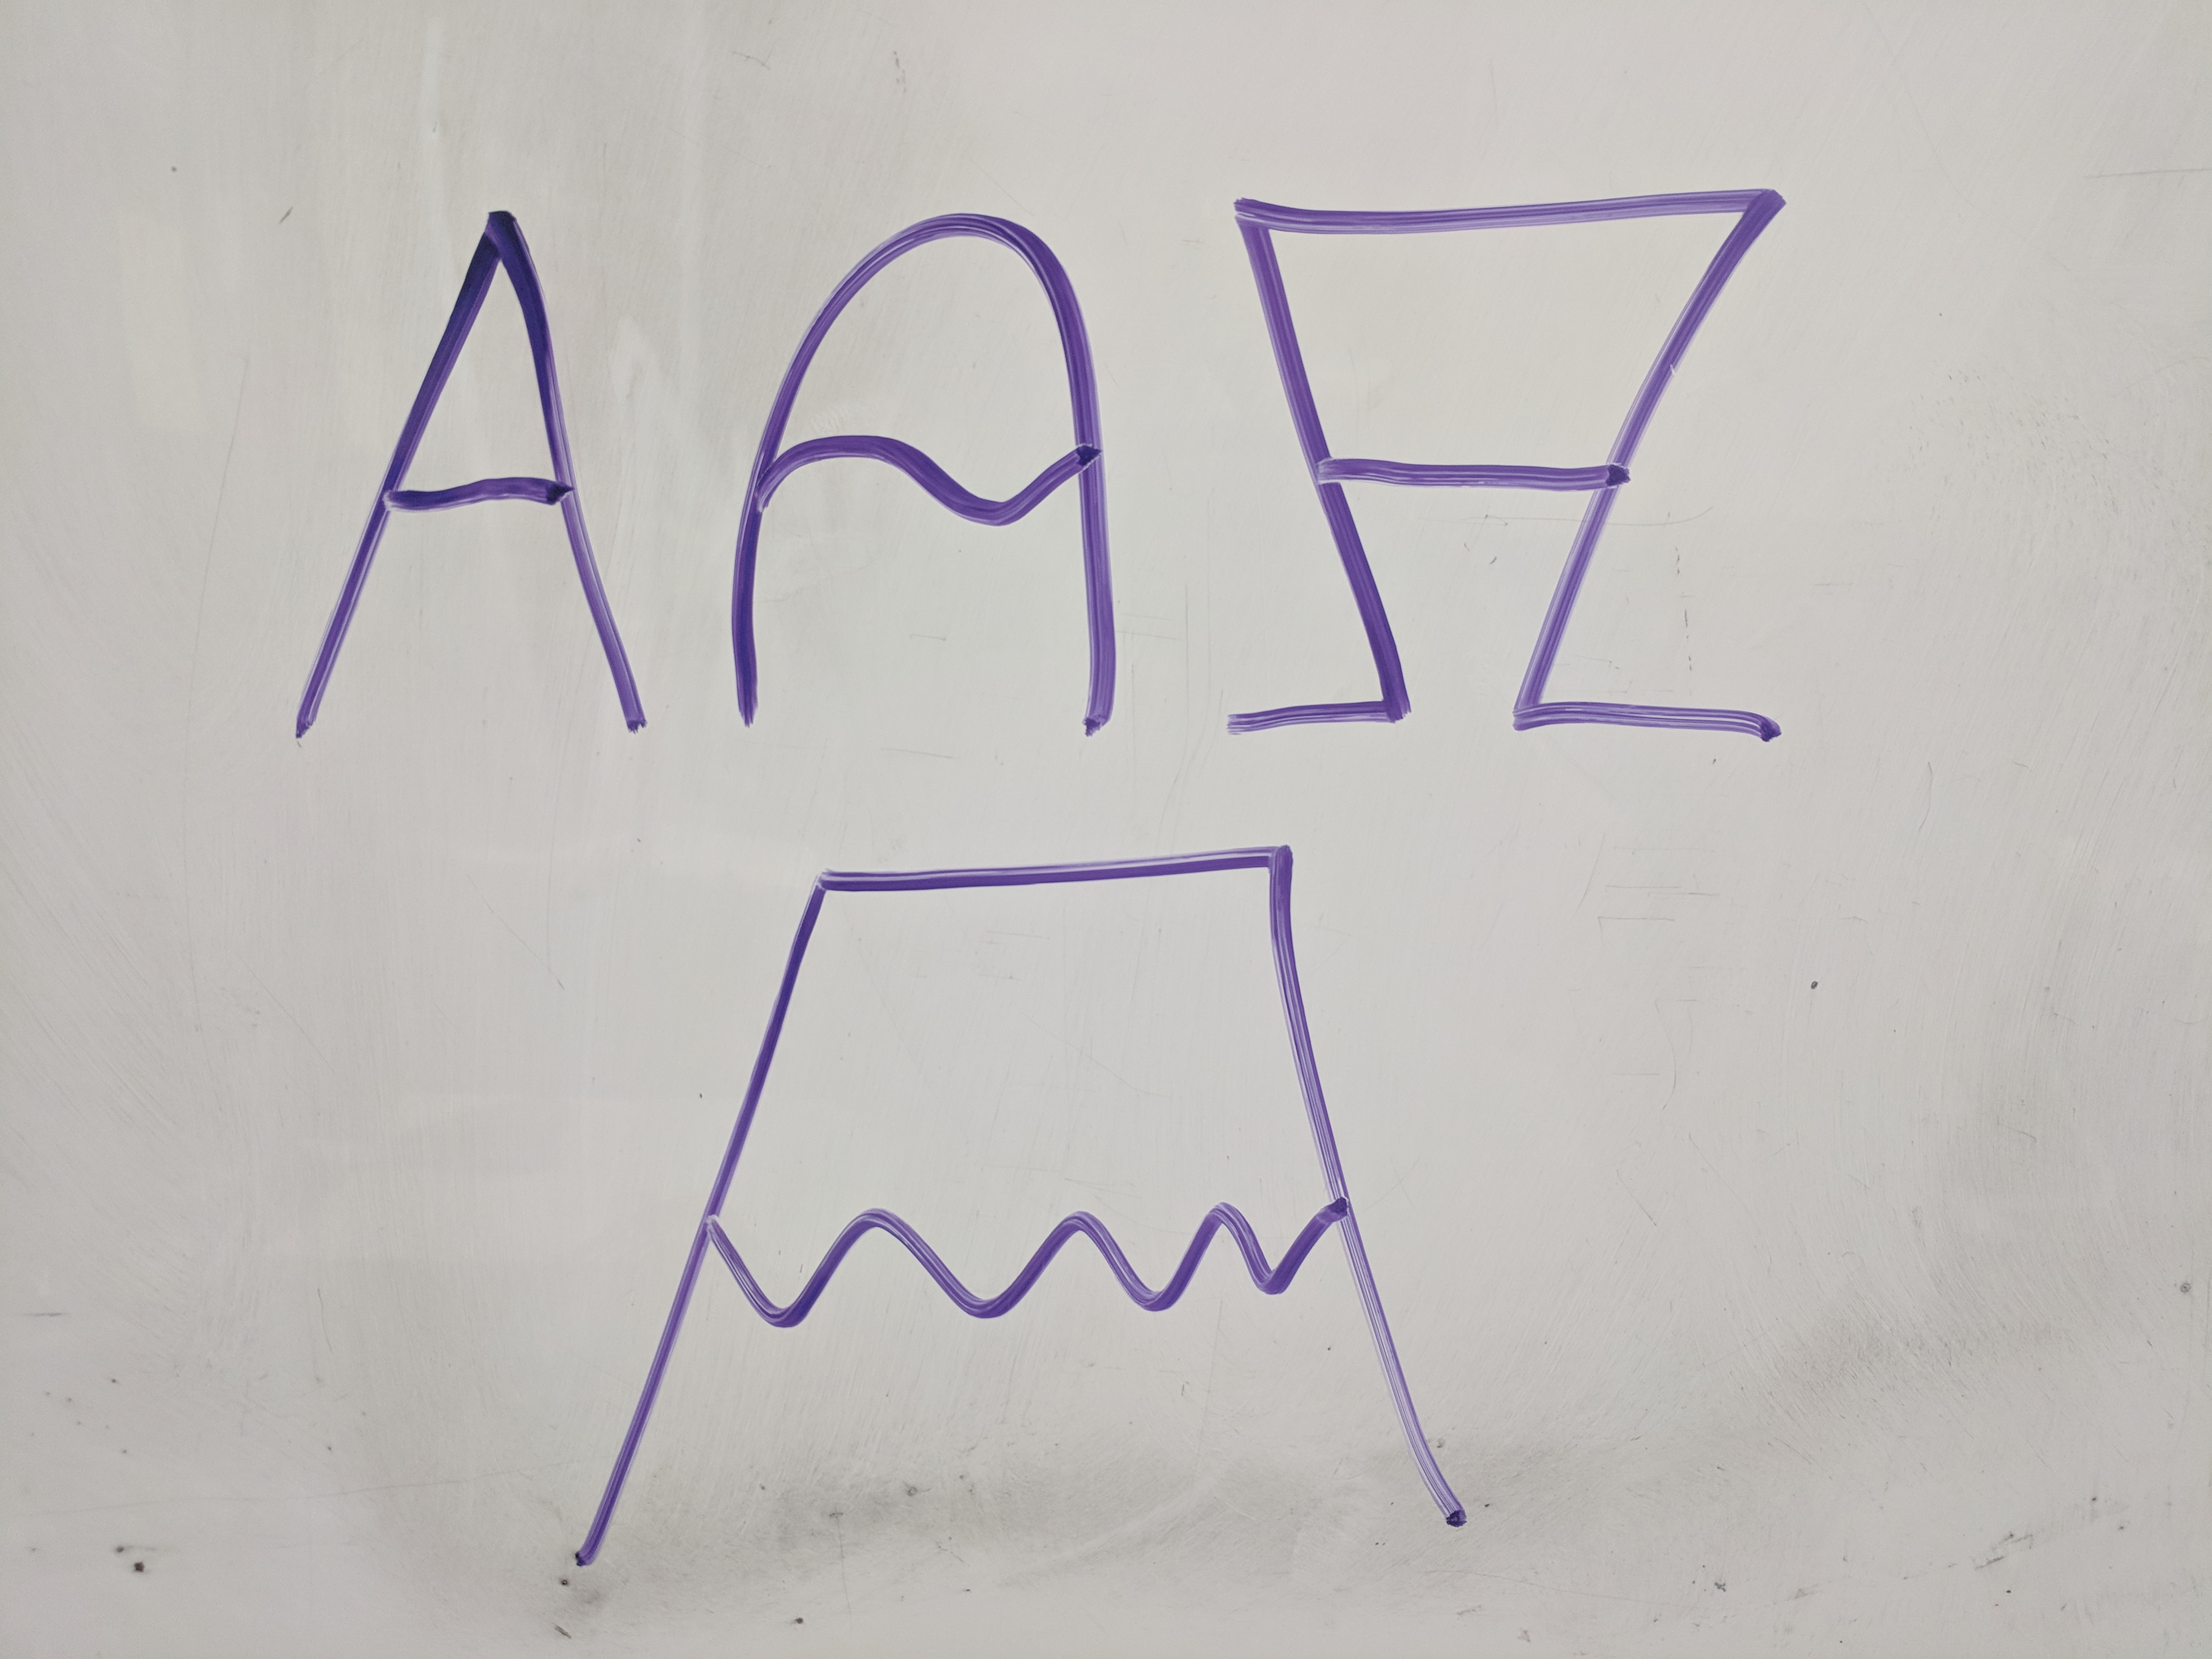
\includegraphics[width=1\linewidth]{images/letter-a.jpg}
\caption{The letter ``A'' in several fonts.\label{figure-letter-a}}
\end{figure}
\hypertarget{p-14}{}%
A homeomorphism is more carefully defined in \hyperref[section-continuity]{Section~\ref{section-continuity}}, but the central idea is that of ``neighborhoods''. For each of the letters ``A'' in \hyperref[figure-letter-a]{Figure~\ref{figure-letter-a}}, note that there are two endpoints and two triad intersections whose neighborhoods look different from the other neighborhoods within the letter; see \hyperref[figure-letter-a-neighborhoods]{Figure~\ref{figure-letter-a-neighborhoods}}.%
\begin{figure}
\centering
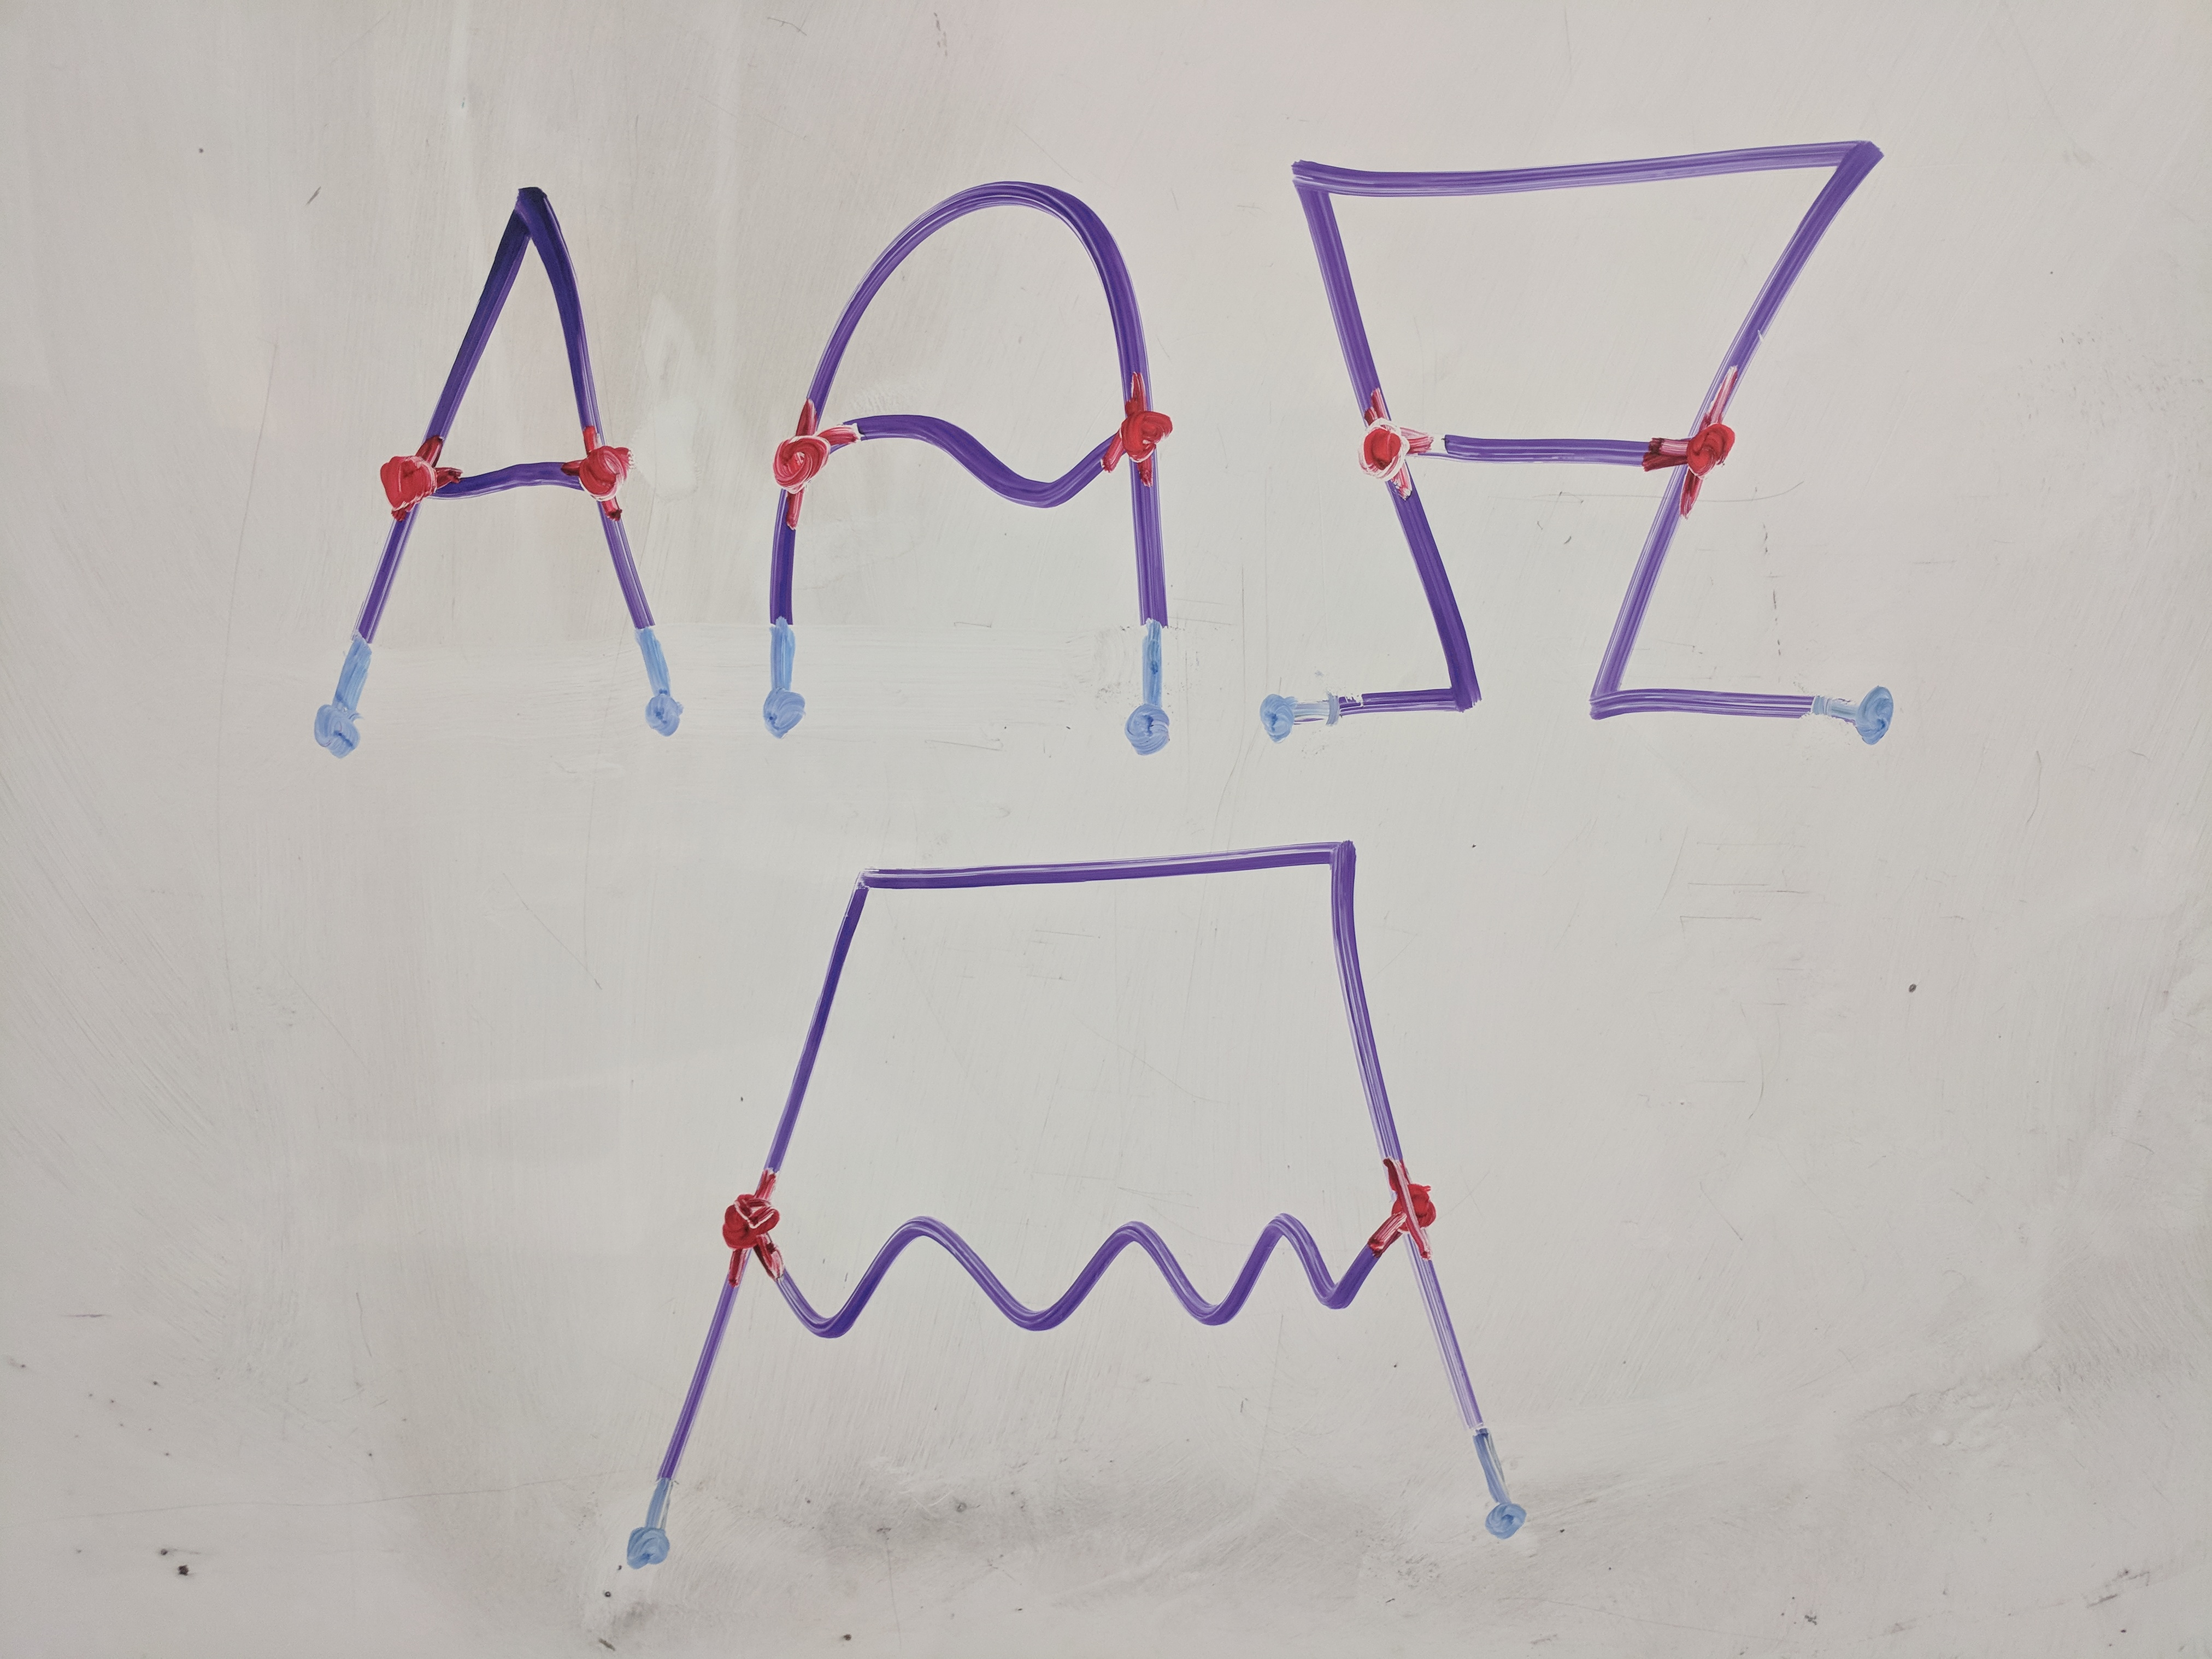
\includegraphics[width=1\linewidth]{images/letter-a-neighborhoods.jpg}
\caption{Neighborhoods within the letter ``A''.\label{figure-letter-a-neighborhoods}}
\end{figure}
\begin{definition}{}{definition-surface}%
\hypertarget{p-15}{}%
A \terminology{surface} is a set of points such that for every point in the set, the set locally looks like a (possibly bent or curved) copy of the plane \(\mathbb R^2\) or the half-plane \(\mathbb R^{2*}=\{\tuple{x,y}\in\mb R^2:x\geq 0\}\).%
\end{definition}
\hypertarget{p-16}{}%
A classic example of the topology of surfaces is the following joke: ``A topologist is a mathematician who cannot tell the difference between his doughnut and coffee cup.'' The joke is a lot funnier\footnote{Eh, maybe.\label{fn-2}} once you've seen \href{https://en.wikipedia.org/wiki/File:Mug_and_Torus_morph.gif}{this animated GIF on Wikipedia}.%
\par
\hypertarget{p-17}{}%
The ``doughnut'''s surface is known mathematically as a ``torus'', shown in \hyperref[figure-torus]{Figure~\ref{figure-torus}}. A sphere is shown in \hyperref[figure-sphere]{Figure~\ref{figure-sphere}}, and a surface that cannot be cannot be embedded in \(\mathbb R^3\), the Klein bottle, is shown in \hyperref[figure-klein-bottle]{Figure~\ref{figure-klein-bottle}}.%
\begin{figure}
\centering
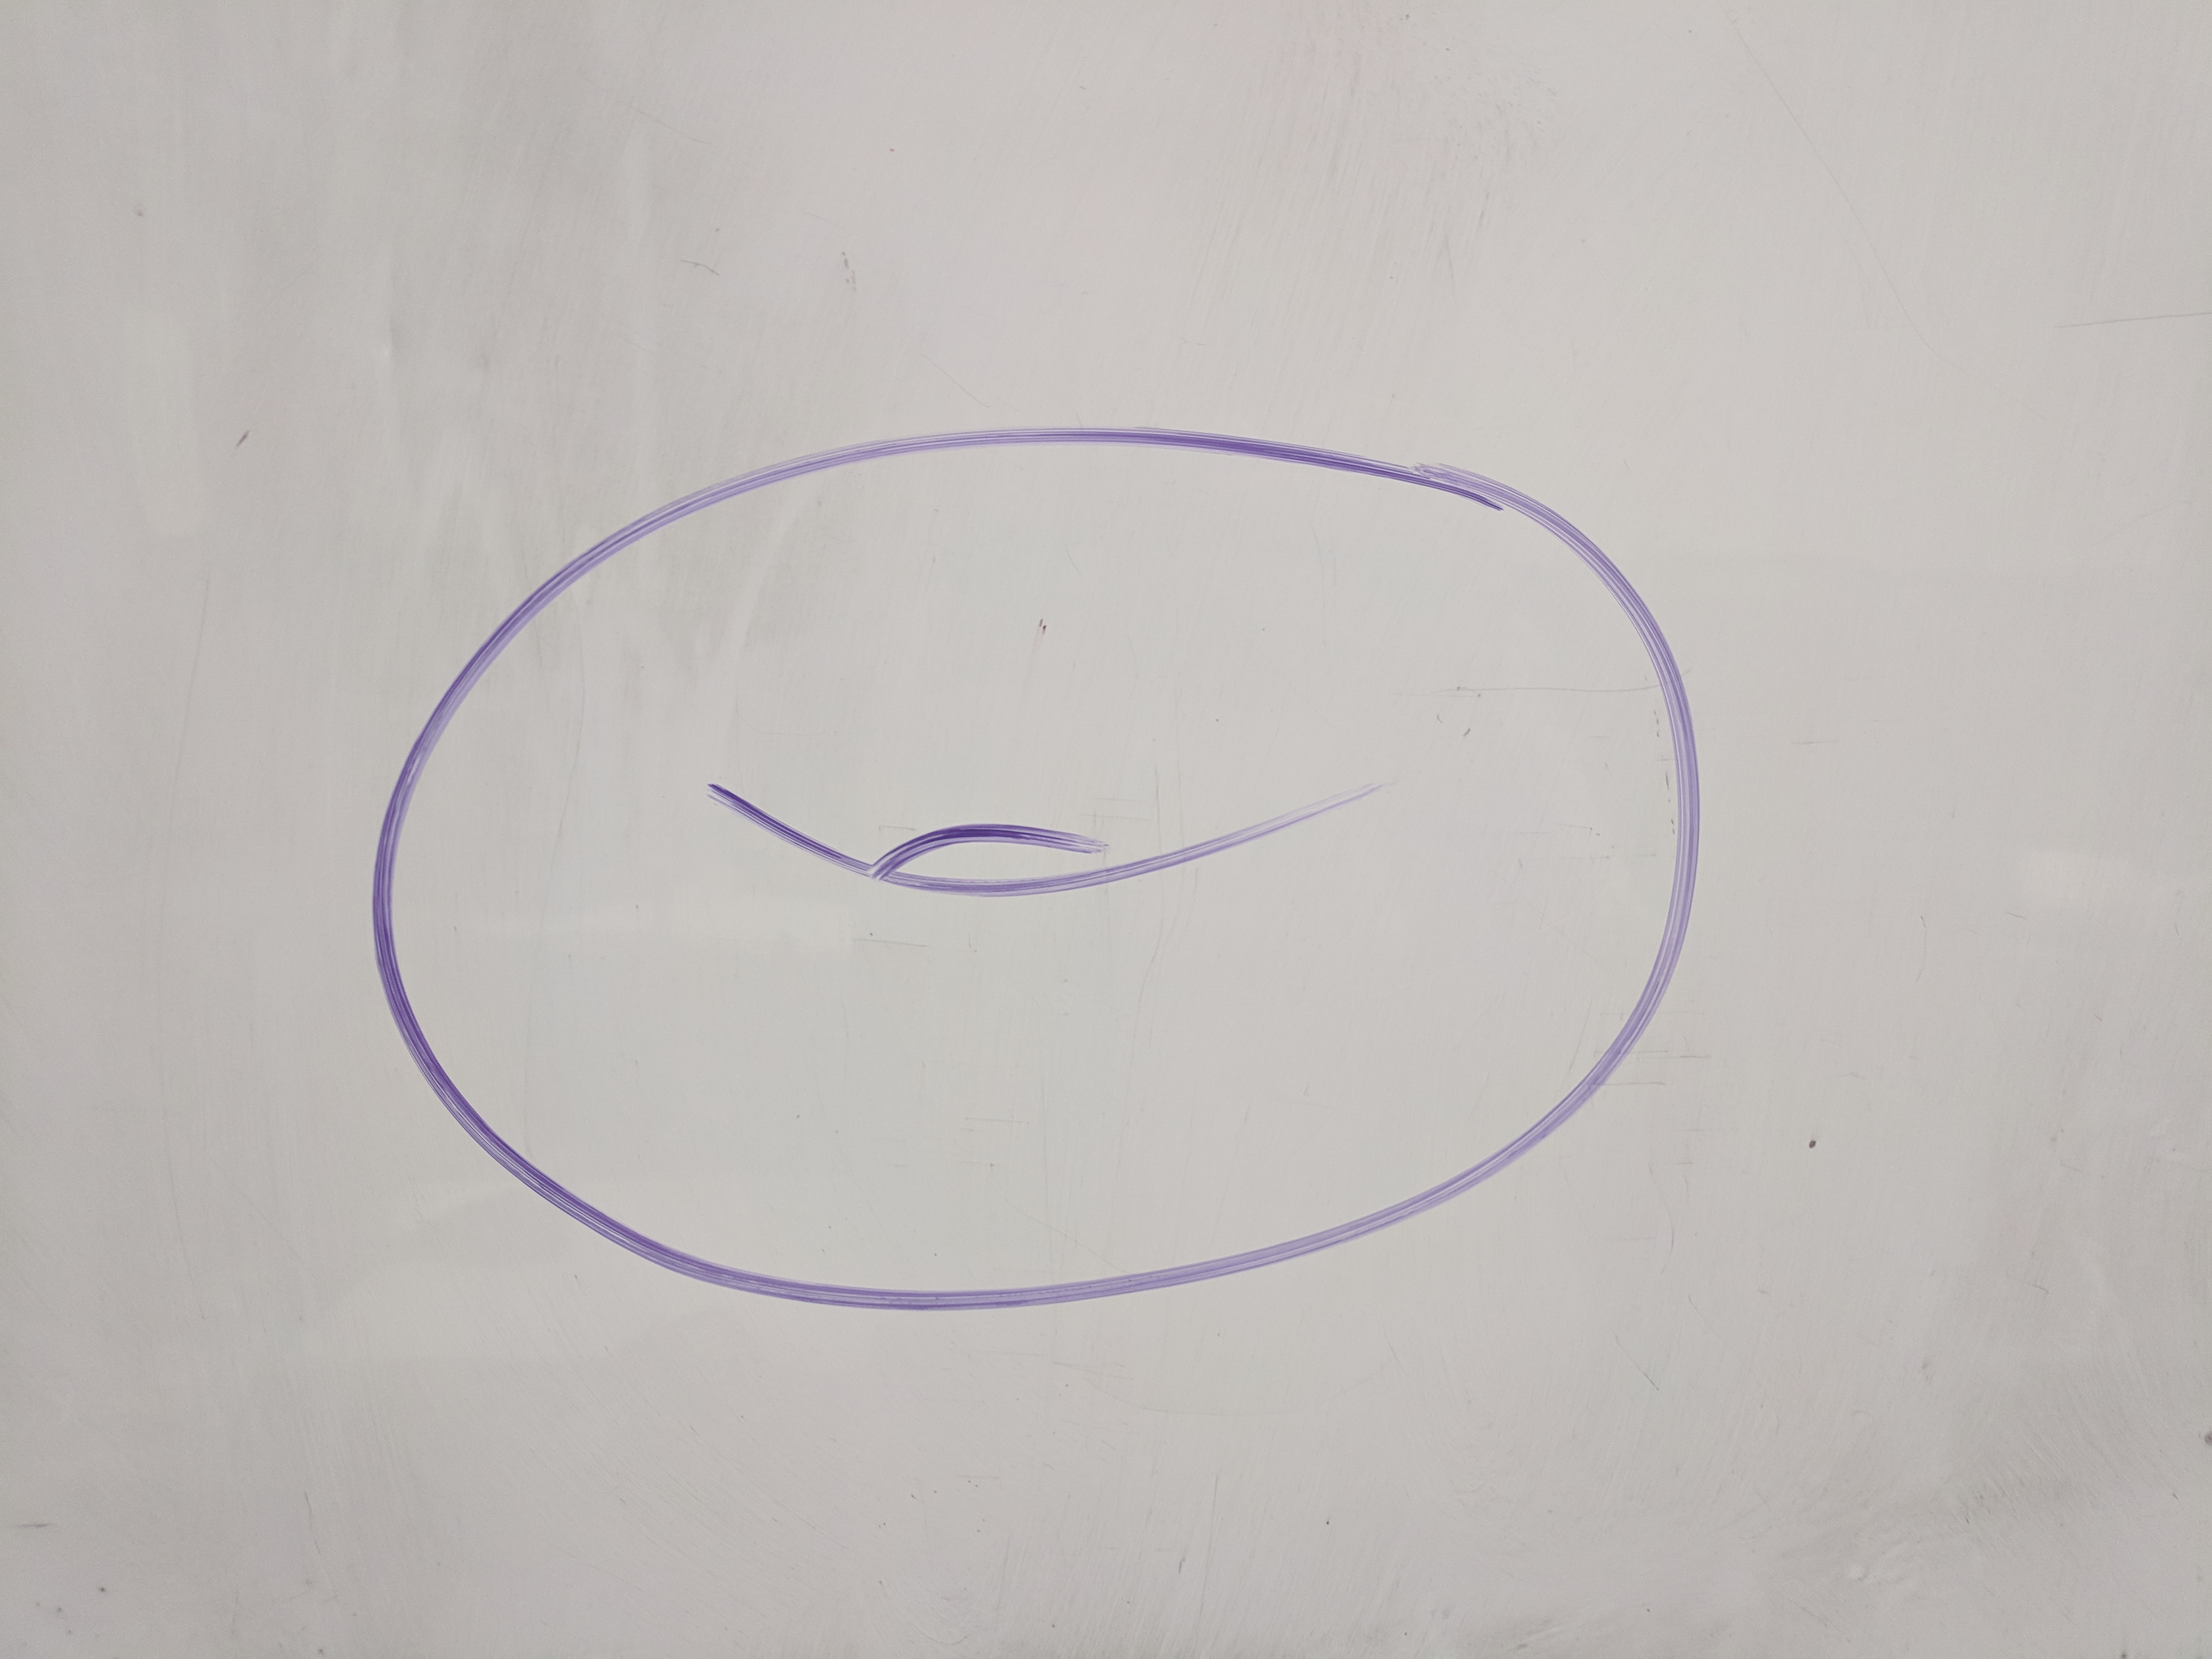
\includegraphics[width=1\linewidth]{images/torus.jpg}
\caption{A torus.\label{figure-torus}}
\end{figure}
\begin{figure}
\centering
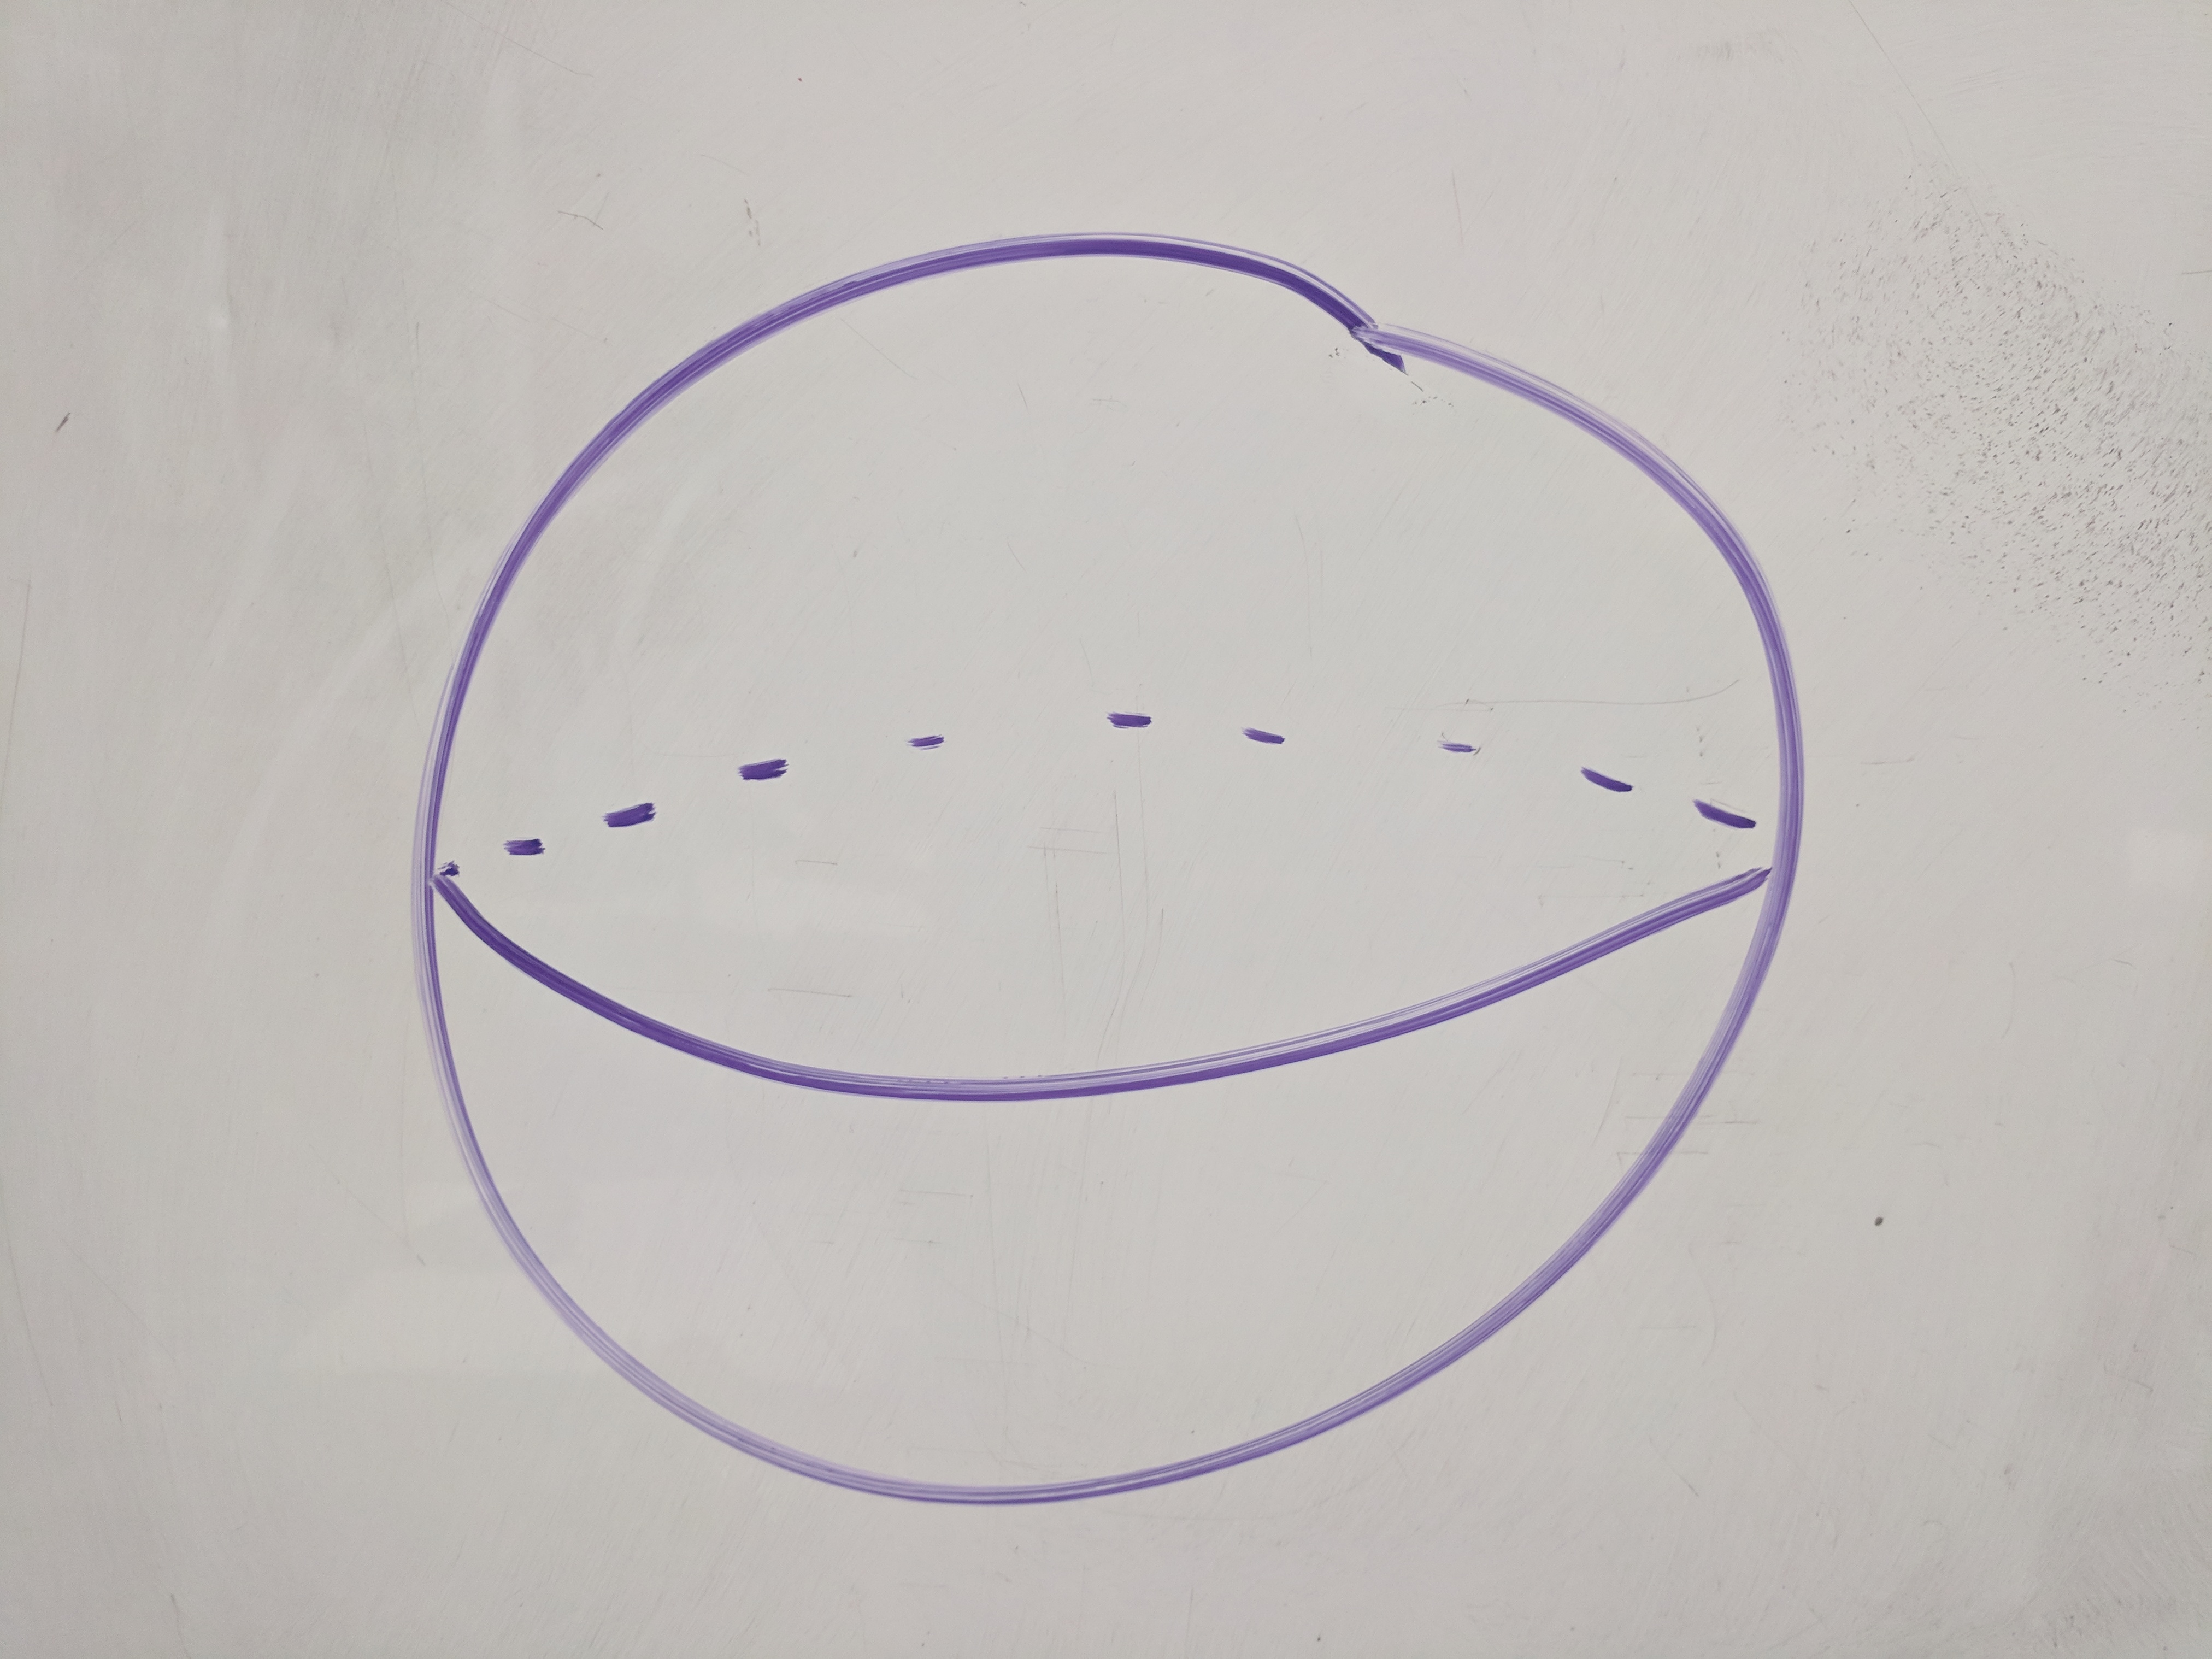
\includegraphics[width=1\linewidth]{images/sphere.jpg}
\caption{A sphere.\label{figure-sphere}}
\end{figure}
\begin{figure}
\centering
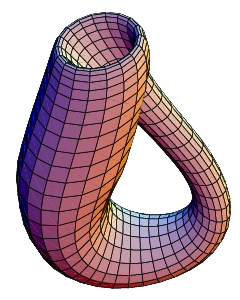
\includegraphics[width=1\linewidth]{images/klein-bottle.png}
\caption{A Klein bottle.\label{figure-klein-bottle}}
\end{figure}
\hypertarget{p-18}{}%
While these shapes appear very different, they can all be defined as a ``quotient space'' (\hyperref[section-quotient-spaces]{Section~\ref{section-quotient-spaces}}) of the unit square in \(\mathbb R^2\).%
\par
\hypertarget{p-19}{}%
In order to study so-called ``topological spaces'' such as these, we will begin by distilling down the notion of a ``neighborhood'' for an arbitrary set.%
%
%
\typeout{************************************************}
\typeout{Section 2 Topological Spaces}
\typeout{************************************************}
%
\section[{Topological Spaces}]{Topological Spaces}\label{section-topological-spaces}
\begin{definition}{}{definition-4}%
\hypertarget{p-20}{}%
Let \(a,b\in\mb R\). The \terminology{open interval} from \(a\) to \(b\) is the set%
%
\begin{equation*}
(a,b)=\setBuilder{x\in\mb R}{a\lt x\lt b}
\end{equation*}
\end{definition}
\begin{definition}{}{limit-point-intro}%
\hypertarget{p-21}{}%
Let \(x\in\mb R\) and \(S\subseteq\mb R\). The point \(x\) is a \terminology{limit point} of the set \(S\) if and only if for every open interval \((a,b)\) containing \(x\), there is a point \(y\in S\) such that \(x\not=y\) and \(y\in(a,b)\).%
\end{definition}
\begin{example}{}{example-1}%
\hypertarget{p-22}{}%
Determine if each set has the number \(0\) as a limit point.%
\leavevmode%
\begin{enumerate}
\item\hypertarget{li-3}{}\(\mb Z\)%
\item\hypertarget{li-4}{}\(\mb R\setminus\mb Z\)%
\item\hypertarget{li-5}{}\(\setBuilder{\frac{1}{n+1}}{n\in\mb N}\)%
\item\hypertarget{li-6}{}\(\mb Q\)%
\item\hypertarget{li-7}{}A finite set \(F\subseteq\mb R\)%
\end{enumerate}
\end{example}
\begin{definition}{}{euclidean-open-sets}%
\hypertarget{p-23}{}%
A subset \(U\subseteq\mb R\) is called \terminology{open} if and only if for every point \(x\in U\), there exists an open interval \((a,b)\) such that \(x\in(a,b)\subseteq U\).%
\end{definition}
\begin{example}{}{example-2}%
\hypertarget{p-24}{}%
Determine if each set is open or not open.%
\leavevmode%
\begin{enumerate}
\item\hypertarget{li-8}{}\([\pi,42)\)%
\item\hypertarget{li-9}{}\((-3,-1)\cup(4,5.5)\)%
\item\hypertarget{li-10}{}\(\setBuilder{x}{2x+1>5}\)%
\item\hypertarget{li-11}{}\(\mb Z\)%
\item\hypertarget{li-12}{}\(\mb R\setminus\mb Z\)%
\item\hypertarget{li-13}{}\(\mb Q\)%
\item\hypertarget{li-14}{}A finite set \(F\subseteq\mb R\)%
\end{enumerate}
\end{example}
\begin{theorem}{}{}{theorem-1}%
\hypertarget{p-25}{}%
A subset \(U\subseteq\mb R\) is open if and only if there exists a collection of open intervals \(\mc U\) such that \(U=\bigcup\mc U\).%
\end{theorem}
\begin{proposition}{}{}{proposition-1}%
\hypertarget{p-26}{}%
Let \(x\in\mb R\) and \(S\subseteq\mb R\). The point \(x\) is a limit point of the set \(S\) if and only if for every open set \(U\) containing \(x\), there is a point \(y\in S\) such that \(x\not=y\) and \(y\in U\).%
\end{proposition}
\begin{theorem}{}{}{euclidean-topology-verification}%
\hypertarget{p-27}{}%
The open subsets of \(\mb R\) satisfy the following properties.%
\leavevmode%
\begin{enumerate}
\item\hypertarget{li-15}{}\(\emptyset\) and \(\mb R\) are open sets.%
\item\hypertarget{li-16}{}If \(\mc U\) is a collection of open sets, then \(\bigcup\mc U\) is also an open set.%
\item\hypertarget{li-17}{}If \(U,V\) are open sets, then \(U\cap V\) is an open set.%
\end{enumerate}
\end{theorem}
\begin{definition}{}{definition-7}%
\hypertarget{p-28}{}%
Let \(X\) be a set, and let \(\mc T\subseteq \mc P(X)\) satisfy the following properties.%
\leavevmode%
\begin{enumerate}
\item\hypertarget{li-18}{}\(\emptyset,X\in\mc T\).%
\item\hypertarget{li-19}{}If \(\mc U\subseteq\mc T\), then \(\bigcup\mc U\in\mc T\).%
\item\hypertarget{li-20}{}If \(U,V\in\mc T\), then \(U\cap V\in\mc T\).%
\end{enumerate}
\hypertarget{p-29}{}%
Then \(\mc T\) is called a \terminology{topology} on \(X\), the pair \(\tuple{X,\mc T}\) is called a \terminology{topological space}, and elements \(U\in\mc T\) are called \terminology{open sets} of the space. (Usually \(\tuple{X,\mc T}\) is abbreviated to just \(X\) when the topology is known from context.)%
\end{definition}
\begin{definition}{}{definition-8}%
\hypertarget{p-30}{}%
Let \(\mc T\subseteq\mc P(\mb R)\) be the collection of open subsets of \(\mb R\) defined by \hyperref[euclidean-open-sets]{Definition~\ref{euclidean-open-sets}}. Then by \hyperref[euclidean-topology-verification]{Theorem~\ref{euclidean-topology-verification}}, \(\mc T\) is a valid topology for \(\mb R\) called the \terminology{Euclidean topology}.%
\end{definition}
\begin{theorem}{}{}{theorem-3}%
\hypertarget{p-31}{}%
Let \(X\) be any set. Then the following sets are topologies on \(X\).%
\leavevmode%
\begin{enumerate}
\item\hypertarget{li-21}{}\(\mc T=\mc P(X)\) is called the \terminology{discrete topology}.%
\item\hypertarget{li-22}{}\(\mc T=\{\emptyset,X\}\) is called the \terminology{indiscrete topology}.%
\end{enumerate}
\end{theorem}
\begin{proposition}{}{}{proposition-2}%
\hypertarget{p-32}{}%
Let \(\mc T\) be a topology, and let \(\mc U\subseteq\mc T\) be finite. Then \(\bigcap\mc U\in\mc T\).%
\end{proposition}
\begin{proposition}{}{}{proposition-3}%
\hypertarget{p-33}{}%
Let \(\mc T\) be the Euclidean topology. There exists a collection \(\mc U=\{U_n:n\in\mb N\}\) such that \(\bigcap\mc U\not\in\mc T\).%
\end{proposition}
\begin{definition}{}{definition-9}%
\hypertarget{p-34}{}%
Let \(a,b\in\mb R\cup\setList{-\infty,\infty}\). The following are called \terminology{intervals} of real numbers.%
%
\begin{equation*}
(a,b)=\setBuilder{x\in\mb R}{a\lt x\lt b}
\end{equation*}
%
\begin{equation*}
[a,b)=\setBuilder{x\in\mb R}{a\leq x\lt b}
\end{equation*}
%
\begin{equation*}
(a,b]=\setBuilder{x\in\mb R}{a\lt x\leq b}
\end{equation*}
%
\begin{equation*}
[a,b]=\setBuilder{x\in\mb R}{a\leq x\leq b}
\end{equation*}
\end{definition}
\begin{example}{}{example-3}%
\hypertarget{p-35}{}%
Show that each of the following is an example of a topological space \(\tuple{X,\mc T}\).%
\leavevmode%
\begin{enumerate}
\item\hypertarget{li-23}{}Let \(X=\mb R\) and \(\mc T=\setBuilder{(x,\infty)}{x\in\mb R\cup\setList{-\infty}}
\cup\setList{\emptyset}\).%
\item\hypertarget{li-24}{}Let \(X=\mb R\) and \(\mc T=\setBuilder{(x,y)}{
x,y\in\mb R\cup\setList{-\infty,\infty} \text{ and }x\lt 0\lt y
}\cup\setList{\emptyset}\).%
\item\hypertarget{li-25}{}Let \(X=\mb R\) and \(U\in\mc T\) if for each \(x\in U\), there exists \(a,b\in\mb R\) such that \(x\in[a,b)\subseteq U\).%
\item\hypertarget{li-26}{}Let \(X=\setList{0,1}\) and \(\mc T=\setList{\emptyset,\setList{0},X}\).%
\item\hypertarget{li-27}{}Let \(X=\mb Z\), \(E=\setBuilder{n\in\mb Z}{n\text{ is even}}\), \(D=\setBuilder{n\in\mb Z}{n\text{ is odd}}\), and \(\mc T=\setList{\emptyset,E,D,X}\).%
\end{enumerate}
\end{example}
\begin{definition}{}{definition-10}%
\hypertarget{p-36}{}%
Let \(\tuple{X,\mc T}\) be a topological space and let \(x\in X\). The set \(N\subseteq X\) is called a \terminology{neighborhood} of \(x\) if and only if there exists an open set \(U\in\mc T\) such that \(x\in U\subseteq N\).%
\end{definition}
\begin{proposition}{}{}{proposition-4}%
\hypertarget{p-37}{}%
A subset \(U\) of a topological space \(X\) is open if and only if \(U\) is a neighborhood of every point it contains.%
\end{proposition}
\begin{definition}{}{definition-11}%
\hypertarget{p-38}{}%
The following are known as \terminology{separation axioms} for a topological space \(\tuple{X,\mc T}\).%
\leavevmode%
\begin{enumerate}
\item\hypertarget{li-28}{}\(\mc T\) is said to be \terminology{\(T_0\)} if and only if for all points \(x,y\in X\) such that \(x\not=y\), there either exists a neighborhood \(U\) of \(x\) such that \(y\not\in U\), or there exists a neighborhood \(V\) of \(y\) such that \(x\not\in U\).%
\item\hypertarget{li-29}{}\(\mc T\) is said to be \terminology{\(T_1\)} if and only if for all points \(x,y\in X\) such that \(x\not=y\), there exist neighborhoods \(U,V\) of \(x,y\) (respectively) such that \(y\not\in U\) and \(x\not\in U\).%
\item\hypertarget{li-30}{}\(\mc T\) is said to be \terminology{\(T_2\)} (also known as \terminology{Hausdorff}) if and only if for all points \(x,y\in X\) such that \(x\not=y\), there exist neighborhoods \(U,V\) of \(x,y\) (respectively) such that \(y\not\in U\), \(x\not\in U\), and \(U\cap V=\emptyset\).%
\end{enumerate}
\end{definition}
\begin{proposition}{}{}{proposition-5}%
\hypertarget{p-39}{}%
\(T_2\Rightarrow T_1\Rightarrow T_0\).%
\end{proposition}
\begin{example}{}{example-4}%
\hypertarget{p-40}{}%
Find or create an example of a topological space \(\tuple{X,\mc T}\) that is:%
\leavevmode%
\begin{enumerate}
\item\hypertarget{li-31}{}Not \(T_0\).%
\item\hypertarget{li-32}{}\(T_0\) but not \(T_1\).%
\item\hypertarget{li-33}{}\(T_1\) but not \(T_2\).%
\end{enumerate}
\end{example}
\begin{theorem}{}{}{theorem-4}%
\hypertarget{p-41}{}%
Let \(X\) be a finite topological space. Then \(X\) is Hausdorff if and only if \(X\) has the discrete topology.%
\end{theorem}
\begin{proposition}{}{}{proposition-6}%
\hypertarget{p-42}{}%
The Euclidean real line is a non-discrete Hausdorff topological space.%
\end{proposition}
\begin{definition}{}{limit-point}%
\hypertarget{p-43}{}%
Let \(S\subseteq X\) be a subset of a topological space. The point \(x\) is a \terminology{limit point} of the set \(S\) if and only if for every neighborhood of \(U\) of \(x\), there is a point \(y\in S\) such that \(x\not=y\) and \(y\in U\).%
\end{definition}
\begin{proposition}{}{}{proposition-7}%
\hypertarget{p-44}{}%
The point \(x\in\mb R\) is a limit point of \(S\subseteq \mb R\) according to \hyperref[limit-point-intro]{Definition~\ref{limit-point-intro}} if and only if it is a limit point according to \hyperref[limit-point]{Definition~\ref{limit-point}} (where \(\mb R\) is assumed to have the Euclidean topology).%
\end{proposition}
\begin{definition}{}{definition-13}%
\hypertarget{p-45}{}%
Let \(S\subseteq X\) be a subset of a topological space. Then \(S'\) is the set of all limit points of \(S\), called the \terminology{derived set} of \(S\).%
\end{definition}
\begin{definition}{}{definition-14}%
\hypertarget{p-46}{}%
Let \(S\subseteq X\) be a subset of a topological space. Then \(\cl S=S\cup S'\) is called the \terminology{closure} of \(S\).%
\end{definition}
\begin{example}{}{example-5}%
\hypertarget{p-47}{}%
Calculate \(\cl S\) for each of the following examples.%
\leavevmode%
\begin{enumerate}
\item\hypertarget{li-34}{}\(S=(-1,1)\subseteq\mb R\) where \(\mb R\) has the Euclidean topology.%
\item\hypertarget{li-35}{}\(S=(-1,1)\subseteq\mb R\) where \(\mb R\) has the discrete topology.%
\item\hypertarget{li-36}{}\(S=(-1,1)\subseteq\mb R\) where \(\mb R\) has the indiscrete topology.%
\item\hypertarget{li-37}{}\(S=\mb Z\subseteq\mb R\) where \(\mb R\) has the Euclidean topology.%
\item\hypertarget{li-38}{}\(S=\mb Q\subseteq\mb R\) where \(\mb R\) has the Euclidean topology.%
\end{enumerate}
\end{example}
\begin{definition}{}{definition-15}%
\hypertarget{p-48}{}%
Let \(H\subseteq X\) be a subset of a topological space. Then \(H\) is called \terminology{closed} if and only if \(H=\cl S\).%
\end{definition}
\begin{theorem}{}{}{theorem-5}%
\hypertarget{p-49}{}%
Let \(H\subseteq X\) be a subset of a topological space. Then \(H\) is closed if and only if there exists an open set \(U\) such that \(H=X\setminus U\).%
\end{theorem}
\begin{proposition}{}{}{proposition-8}%
\hypertarget{p-50}{}%
The closed subsets of a topological space \(X\) satisfy the following properties.%
\leavevmode%
\begin{enumerate}
\item\hypertarget{li-39}{}\(\emptyset\) and \(X\) are closed sets.%
\item\hypertarget{li-40}{}If \(\mc H\) is a collection of closed sets, then \(\bigcap\mc H\) is also a closed set.%
\item\hypertarget{li-41}{}If \(H,L\) are closed sets, then \(H\cup L\) is a closed set.%
\end{enumerate}
\end{proposition}
\begin{theorem}{}{}{theorem-6}%
\hypertarget{p-51}{}%
A topological space \(X\) is \(T_1\) if and only if every finite subset of \(X\) is closed.%
\end{theorem}
\begin{definition}{}{boundary-point}%
\hypertarget{p-52}{}%
Let \(S\subseteq X\) be a subset of a topological space. The point \(x\) is a \terminology{boundary point} of the set \(S\) if and only if for every neighborhood of \(U\) of \(x\), both \(S\cap U\) and \(S\setminus U\) are non-empty.%
\par
\hypertarget{p-53}{}%
Let \(\bd S\) collect all the boundary points of \(S\).%
\end{definition}
\begin{proposition}{}{}{proposition-9}%
\hypertarget{p-54}{}%
Let \(a,b\in\mb R\). Then \(\bd (a,b)=\bd (a,b]=\bd [a,b)=\bd [a,b]=\{a,b\}\) with respect to the Eudlidean topology.%
\end{proposition}
\begin{definition}{}{interior-point}%
\hypertarget{p-55}{}%
Let \(S\subseteq X\) be a subset of a topological space. The point \(x\) is a \terminology{interior point} of the set \(S\) if and only if there exists a neighborhood \(U\) of \(x\) such that \(x\in U\subseteq S\).%
\par
\hypertarget{p-56}{}%
Let \(\int S\) collect all the interior points of \(S\).%
\end{definition}
\begin{proposition}{}{}{proposition-10}%
\hypertarget{p-57}{}%
Let \(U\subseteq X\) be a subset of a topological space. Then \(U\) is open if and only if \(U=\int U\).%
\end{proposition}
\begin{definition}{}{exterior-point}%
\hypertarget{p-58}{}%
Let \(S\subseteq X\) be a subset of a topological space. The point \(x\) is a \terminology{exterior point} of the set \(S\) if and only if there exists a neighborhood \(U\) of \(x\) such that \(x\in U\subseteq X\setminus S\).%
\par
\hypertarget{p-59}{}%
Let \(\ext S\) collect all the exterior points of \(S\).%
\end{definition}
\begin{definition}{}{definition-19}%
\hypertarget{p-60}{}%
A \terminology{partition} of a set \(X\) is a collection \(\mc P\) such that \(X=\bigcup\mc P\) and \(A\cap B=\emptyset\) for all \(A,B\in\mc P\) where \(A\not=B\).%
\end{definition}
\begin{proposition}{}{}{proposition-11}%
\hypertarget{p-61}{}%
Let \(S\subseteq X\) be a subset of a topological space. Then \(\setList{\int S,\bd S,\ext S}\) is a partition of \(X\).%
\end{proposition}
\begin{proposition}{}{}{proposition-12}%
\hypertarget{p-62}{}%
Let \(S\subseteq X\) be a subset of a topological space. Then \(\cl S=\int S\cup\bd S=S\cup\bd S\).%
\end{proposition}
\begin{example}{}{example-6}%
\hypertarget{p-63}{}%
Let \(A\) be a subset of a topological space \(X\). Prove the following.%
\leavevmode%
\begin{enumerate}
\item\hypertarget{li-42}{}\(\int\int A=\int A\)%
\item\hypertarget{li-43}{}\(\int\cl A=\int A\)%
\item\hypertarget{li-44}{}\(\bd\bd A=\bd A\)%
\item\hypertarget{li-45}{}\(\ext\ext A=\int A\)%
\item\hypertarget{li-46}{}\(\int\ext A=\ext A\)%
\item\hypertarget{li-47}{}\(\int\bd A=\emptyset\)%
\item\hypertarget{li-48}{}\(\cl\ext A=X\setminus\int A\)%
\end{enumerate}
\end{example}
\begin{example}{}{example-7}%
\hypertarget{p-64}{}%
Let \(A,B\) be subsets of a topological space \(X\). Prove or disprove the following.%
\leavevmode%
\begin{enumerate}
\item\hypertarget{li-49}{}\(\int(A\cap B)=\int A\cap\int B\)%
\item\hypertarget{li-50}{}\(\int(A\cup B)=\int A\cup\int B\)%
\item\hypertarget{li-51}{}\(\bd(A\cap B)=\bd A\cap\bd B\)%
\item\hypertarget{li-52}{}\(\bd(A\cup B)=\bd A\cup\bd B\)%
\item\hypertarget{li-53}{}\(\cl(A\cap B)=\cl A\cap\cl B\)%
\item\hypertarget{li-54}{}\(\cl(A\cup B)=\cl A\cup\cl B\)%
\end{enumerate}
\end{example}
\begin{definition}{}{definition-20}%
\hypertarget{p-65}{}%
A subset \(D\subseteq X\) of a topological space is called \terminology{dense} if and only if \(\cl D=X\).%
\end{definition}
\begin{example}{}{example-8}%
\hypertarget{p-66}{}%
Determine which of these are dense subsets of \(\mb R\).%
\leavevmode%
\begin{enumerate}
\item\hypertarget{li-55}{}\(\mb Q\)%
\item\hypertarget{li-56}{}\(\mb Z\)%
\item\hypertarget{li-57}{}\(\mb R\setminus\mb Q\)%
\item\hypertarget{li-58}{}\(\mb R\setminus\mb Z\)%
\end{enumerate}
\end{example}
\begin{definition}{}{definition-21}%
\hypertarget{p-67}{}%
The following are also known as \terminology{separation axioms} for a topological space \(\tuple{X,\mc T}\).%
\leavevmode%
\begin{enumerate}
\item\hypertarget{li-59}{}\(\mc T\) is said to be \terminology{regular} if and only if for all points \(x\in X\) and closed subsets \(H\subseteq X\) such that \(x\not\in H\), there exist open sets \(U,V\in\mc T\) such that \(x\in U,H\subseteq V,U\cap V=\emptyset\).%
\item\hypertarget{li-60}{}\(\mc T\) is said to be \terminology{\(T_3\)} if and only if it is both regular and \(T_1\)%
\item\hypertarget{li-61}{}\(\mc T\) is said to be \terminology{normal} if and only if for all closed subsets \(H,L\subseteq X\) such that \(H\cap L=\emptyset\), there exist open sets \(U,V\in\mc T\) such that \(H\subseteq U,L\subseteq V,U\cap V=\emptyset\).%
\item\hypertarget{li-62}{}\(\mc T\) is said to be \terminology{\(T_4\)} if and only if it is both normal and \(T_1\)%
\end{enumerate}
\end{definition}
\begin{proposition}{}{}{proposition-13}%
\hypertarget{p-68}{}%
\(T_{n+1}\Rightarrow T_n\) for \(n\in\setList{0,1,2,3}\).%
\end{proposition}
\begin{theorem}{}{}{theorem-7}%
\hypertarget{p-69}{}%
The real line \(\mb R\) equipped with the Euclidean topology is \(T_4\).%
\end{theorem}
\begin{example}{}{example-9}%
\hypertarget{p-70}{}%
Find or create an example of a topological space that is:%
\leavevmode%
\begin{enumerate}
\item\hypertarget{li-63}{}\(T_2\) but not regular.%
\item\hypertarget{li-64}{}\(T_3\) but not \(T_4\)%
\item\hypertarget{li-65}{}Regular but not \(T_3\).%
\item\hypertarget{li-66}{}Normal but not \(T_4\).%
\item\hypertarget{li-67}{}Regular but not normal.%
\item\hypertarget{li-68}{}Normal but not regular.%
\end{enumerate}
\end{example}
\begin{theorem}{}{}{theorem-8}%
\hypertarget{p-71}{}%
A topological space is \(T_3\) if and only if it is regular and \(T_0\).%
\end{theorem}
\begin{definition}{}{definition-22}%
\hypertarget{p-72}{}%
Let \(\tuple{X,\mc T}\) be a topological space. A subset \(\mc B\subseteq\mc T\) is called a \terminology{basis} for the topology.. TODO.%
\end{definition}
\hypertarget{p-73}{}%
TODO: subspaces, basis and subbasis, first/second countability%
%
%
\typeout{************************************************}
\typeout{Section 3 Continuity \& Homeomorphisms}
\typeout{************************************************}
%
\section[{Continuity \& Homeomorphisms}]{Continuity \& Homeomorphisms}\label{section-continuity}
%
%
\typeout{************************************************}
\typeout{Section 4 Compactness}
\typeout{************************************************}
%
\section[{Compactness}]{Compactness}\label{section-compactness}
%
%
\typeout{************************************************}
\typeout{Section 5 Connectedness}
\typeout{************************************************}
%
\section[{Connectedness}]{Connectedness}\label{section-connectedness}
%
%
\typeout{************************************************}
\typeout{Section 6 Metric Spaces}
\typeout{************************************************}
%
\section[{Metric Spaces}]{Metric Spaces}\label{section-metric-spaces}
%
%
\typeout{************************************************}
\typeout{Section 7 Product Spaces}
\typeout{************************************************}
%
\section[{Product Spaces}]{Product Spaces}\label{section-product-spaces}
%
%
\typeout{************************************************}
\typeout{Section 8 Quotient Spaces}
\typeout{************************************************}
%
\section[{Quotient Spaces}]{Quotient Spaces}\label{section-quotient-spaces}
%
%
\typeout{************************************************}
\typeout{Appendix A Naive Set Theory}
\typeout{************************************************}
%
%
\appendix
%
\section[{Naive Set Theory}]{Naive Set Theory}\label{set-theory}
\hypertarget{p-74}{}%
A review of basic results concerning sets.%
\begin{definition}{}{definition-23}%
\leavevmode%
\begin{itemize}[label=\textbullet]
\item{}\(\mb R\) is the set of real numbers.%
\item{}\(\mb Z\) is the set of integers.%
\item{}\(\mb N=\setBuilder{z\in\mb Z}{z\geq 0}=\setList{0,1,2,\dots}\) is the set of natural numbers, which includes zero.%
\item{}\(\mb Q=\setBuilder{\frac{z}{n+1}}{z\in\mb Z,n\in\mb N}\) is the set of rational numbers.%
\end{itemize}
\end{definition}
\begin{theorem}{}{}{theorem-9}%
\hypertarget{p-75}{}%
The \terminology{Archemedian Property} of the real numbers guarantees that for each real number \(x\in\mb R\), there exists a natural number \(n\in\mb N\) such that \(\frac{1}{n}\lt x\).%
\end{theorem}
\begin{theorem}{}{}{theorem-10}%
\hypertarget{p-76}{}%
\terminology{De Morgan's Laws}: Let \(\mc A\) be a collection of subsets of \(X\).%
%
\begin{equation*}
X\setminus\bigcup_{A\in\mc A}A=\bigcap_{A\in\mc A}(X\setminus A)
\end{equation*}
%
\begin{equation*}
X\setminus\bigcap_{A\in\mc A}A=\bigcup_{A\in\mc A}(X\setminus A)
\end{equation*}
\end{theorem}
\end{document}